\chapter{GSM}
\label{ch:gsm}
This chapter will give a short overview of some important aspects of \gls{gsm} networks and protocols.
The first section presents a brief historical summary on the evolution of \gls{gsm} and how it came to be what it is today.
In Section \ref{sec:network} the system architecture and its components as well as essential protocol basics will be explained, important to understand which place in the network an IMSI-catcher tries to take over.
The $U_m$ interface will be described in detail in Section \ref{sec:Um} since this is the main source for gathering information from IMSI-catchers.
Section \ref{sec:catcher} will finally explain how an IMSI-catcher works and how it replaces the system components as well as state from a technical and law perspective why these devices have become a threat to all-day privacy. 
 
\section{A Historical Perspective}
The acronym GSM was originally derived fom \emph{Group Sp\'{e}ciale Mobile}.
This committee was part of the \gls{cept} 1982, with the task of developing a pan-Eurpean digital cellular mobile radio standard in the 900 MHz band.
1986 the frequency range was officially licensed.
The foundation of this task group was a direct answer to the development of independent and incompatible analog radio networks during the 80's.
Examples of such networks were the C-Netz in Germany, the \gls{tacs} in the UK and \gls{nmt} in Scandinavia.

In February 1987 the committee submitted the basic parameters of GSM. 
Not after after, in September, the \gls{MoU} was signed in Copenhagen by 15 members of 13 Countries that were dedicated to deploy GSM in their respective countries.
This agreement was the foundation for allowing international operation of mobile stations using the standard interfaces agreed upon earlier that year.
\gls{cept} itself was around since 1959 and its members founded the \gls{etsi} in 1988.
In the same year the committee submitted the first detailed specification for the new communications standard.
The acronym was reinterpreted in 1991 after the committee became a part of the \gls{etsi} in 1989 to \emph{Global System for Mobile Communications}.
The very same year the specifications for \gls{dcs1800} were submitted.
These were essentially the same specifications translated to the 1800 MHz band and the foundation for the USA's 1900 MHz band.
Under the umbrella of the \gls{etsi}, many \glspl{stc} began to work on different aspects of mobile communication, like network aspects (SMG 03) or security aspects (SMG 10).
SMG 05 dealt with future networks and especially with UMTS specifications which eventually became an independent body inside the \gls{etsi}.

In 1992 many European countries had operational mobile telephone networks.
These networks were a huge success, and as early as 1993 they already counted more than one million subscribers \cite{GSM2009}.
Also many networks on different frequency bands (900 MHz, 1800 MHz, 1900 MHz) were started outside Europe in countries like the US or Australia with Telstra as the first non European provider.
The rapid growth of mobile subscribers worldwide until today can be seen in figure \ref{fig:gsm_growth}.
Three of the main reasons for this rapid growth are explained by Heine \cite{protocols1999} as:
\begin{itemize}
	\item Liberalisation of the mobile market in Europe which allowed for competition and thus resulting in lower prices and enhanced development.
	\item Expertise within the Groupe Sp\'{e}ciale Mobile and their collaboration with industry.
	\item The lack of competitive technologies.
\end{itemize}

\begin{figure}
\centering
\begin{tikzpicture}
\begin{axis}[
	width=\textwidth,
	height=0.3\textheight,
	xlabel=Year, 
	ylabel=Subscribers,
	xticklabel style={/pgf/number format/1000 sep=}
	]
	\addplot [smooth,mark=*,blue] plot coordinates {
		(1994, 1e6)
		(1995, 10e6)
		(1996, 50e6)
		(1998, 100e6)
		(2001, 500e6)
		(2005, 1.5e9)
		(2007, 2.5e9)
		(2008, 3e9)
		(2009, 3.5e9)
		(2010, 3.7e9)
		(2011, 4e9)
	};
\end{axis}
\end{tikzpicture}
\caption{Growth of mobile GSM subscriptions. Compiled from \cite{GSM2009,GSM_history2011,GSM_stats2011}}
\label{fig:gsm_growth}
\end{figure}

%\begin{figure}
%\centering
%
\includegraphics[width=.5\textwidth]{../Images/3gpp.jpg}
%\caption{The 3GPP Logo}
%\end{figure}

In 1998 the \gls{3gpp} was founded by five organisational partners with the goal of standardisation of mobile communications with focus on developing specifications for a third generation mobile radio system.
These partners were the \gls{arib}, the \gls{etsi}, the \gls{atis}, the \gls{tta} and the \gls{ttc}.
The focus was later expanded in the light of the \emph{International Mobile Communications-2000}-project \cite{3gpp_Proposal2000} by the \gls{itu} to:
\begin{itemize}
	\item Development and maintenance of \gls{gsm} and \gls{gprs}, including \gls{edge}, which are standards for high speed packet oriented data transmission via \gls{gsm}.
	\item Development of a third generation mobile communication system on the basis of the old \gls{gsm} protocol. This standard is called \gls{umts}.
	\item An IP based multimedia system.
\end{itemize}
Up to now the \gls{3gpp} has enhanced mobile standards.
In 2005 the first \gls{hsdpa} network went online.
\gls{hsdpa} \cite{hsdpa} is a protocol that enables mobile users to download data with speeds up to 84 MBit/s since release 9.
\gls{hsupa} \cite{hsupa} is a related protocol in the \gls{hspa} family that provides similar functionality for uploading data.
These and other specification are published on the \gls{3gpp} website\footnote{\url{http://www.3gpp.org/}}.

\section{The GSM Network}
\label{sec:network}

The \gls{gsm} network is a distributed, star shaped network that is built on top of existing telephony infrastructure to additionally connect mobile users.
The telephony network is not only used to connect mobile subscribers to landline phones but also to connect the different components of the mobile network.
The main components of a \gls{gsm} network can be seen in Figure \ref{fig:gsm_network} as well as the interfaces that are used to connect them.
\begin{figure}
\centering
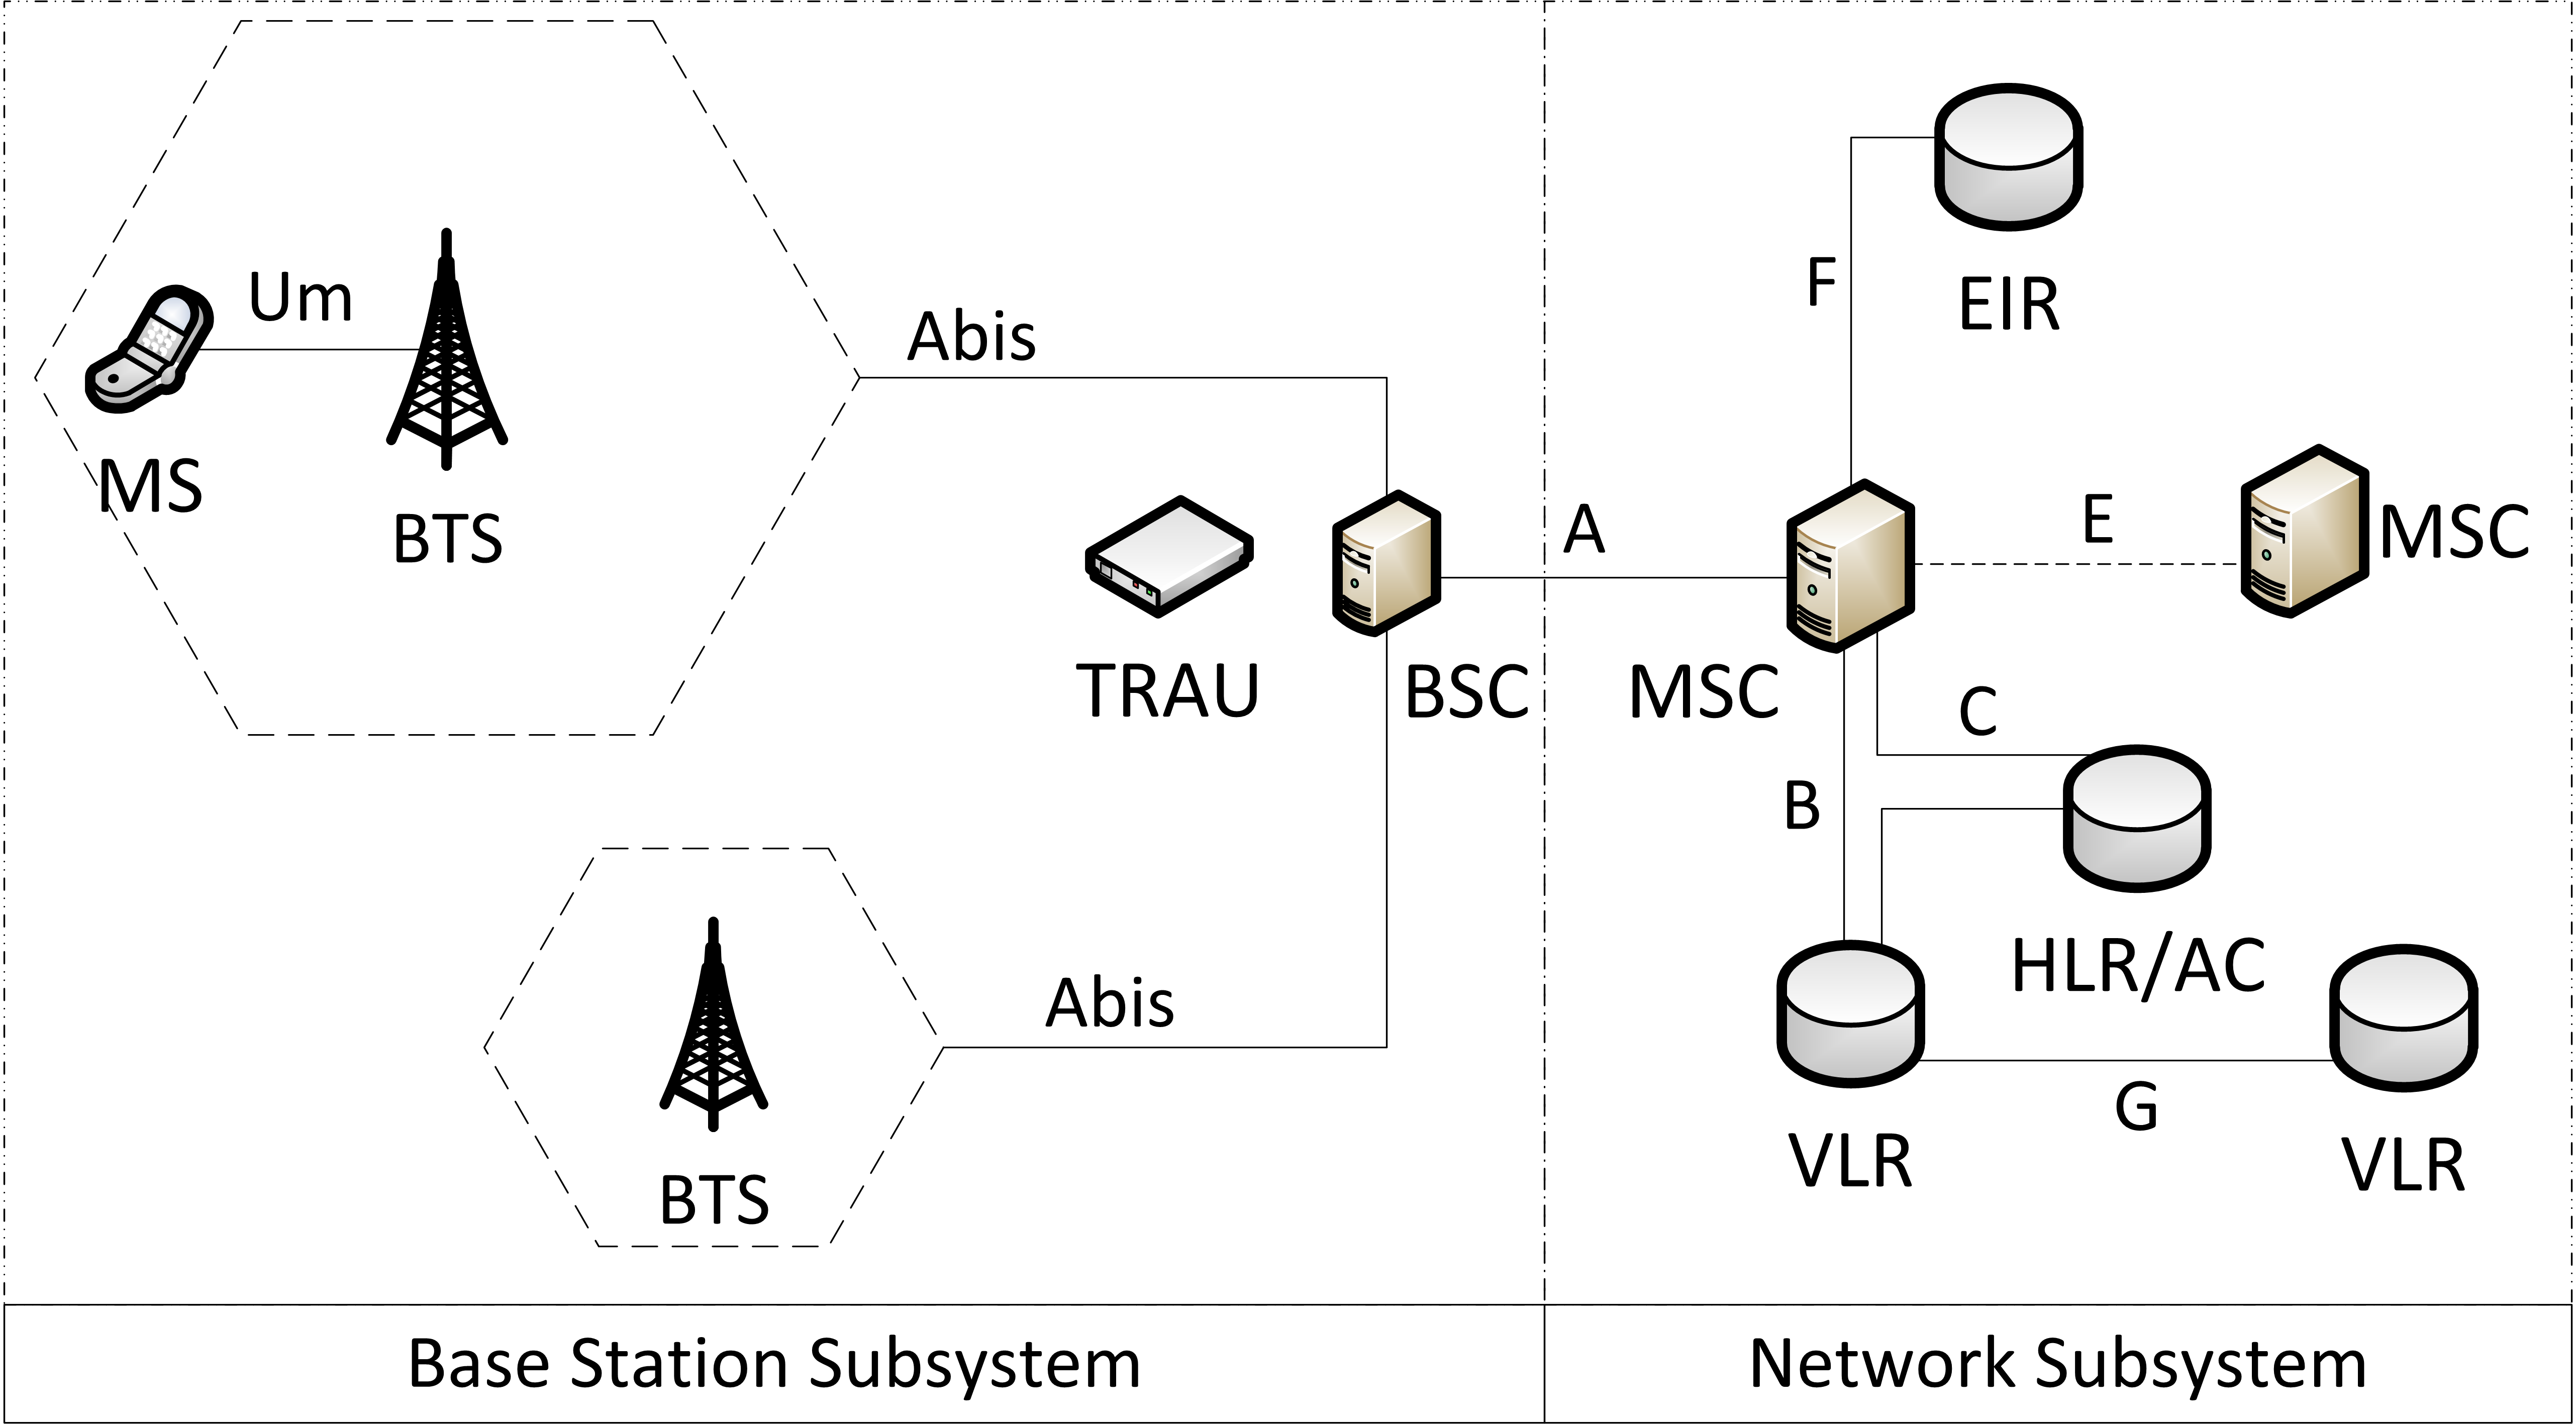
\includegraphics{../Images/Architecture}
\caption{The main components of a GSM network.}
\label{fig:gsm_network}
\end{figure}
There are different notions of how to distribute these components into functional entities.
In the following the classification by Sauter \cite{kommsys2006} will be used.
It describes the main parts as:
\begin{itemize}
	\item \textbf{\gls{bss}:} this part is also called radio network and contains all the technology necessary for connecting mobile subscribers to the telephone network and routing their calls. 
	These calls originate from the \gls{ms} that will be explained in section \ref{sec:ms}, and travel over the air interface to the receiver stations for further processing.
	The air interface or $U_m$ interface will be explained in section \ref{sec:Um}, whereas the rest of the subsystem will be discussed in section \ref{sec:bss}.
	\item \textbf{\gls{nss}:} the core network, as it is sometimes called, consists of several entities that are used to establish and route a connection.
	This is not only limited to calls within the provider's network but also into other provider's networks or the \gls{pstn}.
	The databases that contain subscriber information and location information for connected users are located here.
	\item \textbf{\gls{in}:} this part of the network augments the core network with \gls{vas} \cite{ITU1200}.
	In order to provide extra functionality the \gls{in} consists of several \gls{scp} databases.
	Some of the most widely used services are in fact services of the \gls{in} and not core services.
	Examples are prepaid cards, home areas\footnote{This service defines a geographical area, in which lower rates are calculated for mobile calls.} or telephone number portability.
\end{itemize}
Other sources define the \gls{oms} \cite{GSM2009} or limit the \gls{bss} entity to the provider part and define an additional entity for the \gls{ms} \cite{overview1994, overview1996}.
The three subsystems as well as the \gls{ms} will now be discussed in greater detail.

\subsection{Mobile Station}
\label{sec:ms}
With the advent of portable microprocessors in the 80's mobile phones became possible.
Advance in technology up to today yielded ever smaller mobile phones with ever more functionality year by year to a point where not the technology itself was the constraining factor for size but the user interface, \eg button and display sizes.
What hasn't changed is the basic distinction between \gls{me} and \gls{sim}, the parts of which a \gls{ms} consists.

It is hard to deliver a consistent definition for what a \gls{me} is.
GSM Recommendation 02.07 \cite{GSM0207} summarizes the mandatory and optional features of a \gls{ms}.
Some of the most important mandatory features are \cite{protocols1999}:
\begin{itemize}
	\item \gls{dtmf} signaling capability.
	\item \gls{sms} capability.
	\item The ciphering algorithms A5/1 and A5/2 need to be implemented.
	\item Display capability for short messages and dialed numbers, as well as available \gls{plmn}s.
	\item Capable of doing emergency calls without \gls{sim} card.
	\item Machine fixed \gls{imei}.
	In a strict sense this disqualifies many modern mobile phones since the \gls{imei} is not fixed onto the device itself but rather is part of the software or firmware.
	Tools like \emph{ZiPhone}\footnote{\url{http://www.ziphone.org/}} for iOS devices\footnote{\url{http://www.apple.com/ios/}}, especially iPhone, can change this supposedly unchangeable identifier.
\end{itemize}

The range of devices complying to these specifications is rather large so finding a categorisation can be challenging.
The intuitive approach would be to establish buckets by device type but there are so many different devices as well as hybrid devices out there that this approach would be impracticable.
Does a smartphone belong into the same category as a \gls{pda} or in the category of basic mobile phones; and what would a basic mobile phone be?

Another way to categorize different \gls{me}s is by supported frequency band and power class rating according to GSM  05.05\cite{GSM0505}.
Most mobile phones and smartphones belong to power class 4 and 5, which are for handheld devices.
Class 4 devices have and output of 2/33 W/dBm and class 5 0.8/29 W/dBm.
Classes with higher output are typically installed devices, \eg in cars.
These classes are different for each of the frequency bands, since output needed in higher frequency bands (1800/1900 MHz) is less compared to the 900 MHz band, or the north American 850 MHz band.

The supported band is also common category, since it describes in which countries a mobile phone can be used.
However it is more common nowadays that \gls{me} supports two bands, three bands or even all four bands.
These are called dual-band, tri-band and quad-band devices respectively.

As the name suggests the \gls{sim} card is essentially a data storage that holds user specific data.
This separation is interesting for the GSM user since it allows him/her to exchange the \gls{me} without having to contact the provider.
Thus it can be used on different frequency bands and is one of the preconditions for roaming.
The \gls{sim} card can either be in plug-in format or ID-1 SIM format which is normally used for telephone cards, credit cards or car installed \gls{me}.
The plug-in format is also called ID-000 and can be found in ISO/IEC 7810\cite{ISO7810}.

The most important information stored on a \gls{sim} card are the \gls{imsi} and the \gls{ki}.
A subset of other parameters stored on the \gls{eeprom} of the card can be seen in Table \ref{tab:simdata}.

\begin{table}
\centering
\begin{tabular}{@{}l>{\raggedright\arraybackslash}p{.8\textwidth}@{}}
\toprule
Parameter		&Description\\
\midrule
\multicolumn{2}{l}{Security Related}\\
\midrule
A3/A8			&Algorithms required for authentication and generation of the session key\\
Ki				&Secret key\\
Kc				&Session key, generated from a random number and Ki vie A8\\
PIN				&Secret numeric password to use a SIM card\\
PUK				&Secret numeric password to unlock the SIM card\\
\midrule
\multicolumn{2}{l}{Subscriber Data}\\
\midrule
IMSI			&Subscriber identification\\
MSISDN			&Telephone number\\
\midrule
\multicolumn{2}{l}{Network Related}\\
\midrule
LAI				&Identifier of the current location area\\
TMSI			&Temporary IMSI\\
Home PLMN		&Multiple entries to identify the home PLMN\\
\bottomrule
\end{tabular}
\caption{Subset of data stored on a SIM card. Adopted from \cite{protocols1999}}
\label{tab:simdata}
\end{table}

This key is used to generate the \gls{kc}, as will be explained in Section \ref{sec:nss}.
Most of this data, although not the security relevant \gls{ki} can be read via a USB \gls{sim} card reader, which can be bought for around \$10 on the web.
Since \gls{ki} never leaves the card, \gls{kc} has to be dynamically generated on the card.
This can be done since the card itself has a microprocessor that manages the security relevant data.
Key functions, like running the GSM key algorithm, verifying a \gls{pin} or reading a file can be accessed through the microprocessor via a communication protocol.
A brief description of the protocol and functionalities can be found in Sauter's book \cite{kommsys2006}.

The \gls{imsi} as described in GSM 23.003\cite{GSM23003} uniquely identifies a subscriber.
It has at most 15 digits and is divided into three parts, \gls{mcc}, \gls{mnc} and \gls{msin} of which only the last part is the personal identification number of the subscriber.
The first two are also called \gls{hni}.
The three digit \gls{mcc} describes the country code, the area of domicile of the mobile subscriber.
The \gls{mnc} is an identification number for the home \gls{plmn}.
This can either have two or three digits depending on the \gls{mcc}.
It is not recommended by the specification and thus not defined to mix two and three digit \gls{mnc}s for a single \gls{mcc}.
These country codes are assigned by the \gls{itu} in ITU E.212 \cite{ITU212}.
An excerpt can be found in Table \ref{tab:countrycodes}.
The third part, the \gls{msin} is a number consisting of up to ten digits which is used for authentication of the mobile subscriber against his provider.
\gls{mnc} and \gls{msin} together are called \gls{nmsi}.
\begin{table}
\centering
\subtable{
\begin{tabular}{ll}
\toprule
Country		&MCC\\
\midrule
Germany		&262\\
France		&208\\
USA			&310 - 316\\
UK			&234 - 235\\
Switzerland	&228\\
Austria		&232\\
Poland		&260\\
\bottomrule
\end{tabular}
}
\hspace{.5cm}
\subtable{
\begin{tabular}{lll}
\toprule
Provider	&Country		&MNC\\
\midrule
T-Mobile	&Germany		&01, 06(R)\\
Vodafone	&Germany		&02, 04(R), 09(R)\\
E-Plus		&Germany		&03, 05(R), 77(T)\\
$O_2$		&Germany		&07, 08(R), 11(R)\\
Orange		&France			&00, 01, 02\\
Swisscom	&Switzerland	&01\\
A1			&Austria		&01, 09\\
\bottomrule
\end{tabular}
}
\caption{Mobile Country and Network Codes. (R) denotes that the MCC is reserved but not operational as of yet, whereas (T) denotes a operational test network.}
\label{tab:countrycodes}
\end{table}

\subsection{Network Subsystem}
\label{sec:nss}
The most important task of the Network Subsystem or Network Switching Subsystem is to establish connections and route calls between different locations.
This is done by so called \gls{msc} that can route a call either to another \gls{msc}, into the \gls{pstn} or another provider's network.
Apart from routing, the \gls{nss} also provides the means to administer subscribers inside the network.
Facilities to support this task are the \gls{hlr}, the \gls{vlr}, the \gls{eir} as well as the \gls{ac}.
These will now be described in further detail.
The \gls{smsc} is also part of this subsystem handling text messages.
A possible arrangement of these components is displayed in Figure \ref{fig:gsm_network}.

\subsubsection{Mobile Switching Center}
The \gls{msc} is the component that does the actual routing of calls and therefore is the core component of the \gls{nss}.
It basically works like any other \gls{isdn} exchange device with additional functionality to manage mobility.
Since the amount of signalling inside a \gls{plmn} would be far to big for a single \gls{msc} there is one for every \gls{la}.
Amongst others its most important tasks are \gls{cc} and \gls{mm}.

\gls{cc} entrails registration when the subscriber connects to the network as well as routing the calls or text messages from one registered subscriber to another. 
This routing can include transmission of calls to landlines or to networks of other providers.
\glspl{msc} that bind the provider's networks to other providers' networks or the \gls{pstn} are called Gateway \glspl{msc}.

The above part is also true for pure landline switching centres.
What sets a mobile switching centre apart from these is called \gls{mm}.
Since the participants can freely move around the network  and thus cannot be identified the same way as a fixed landline participant, authentication before using the offered services is important.
Another consequence of mobility is that the network has to keep track of where a subscriber is and through which \gls{msc} it can be reached.
This is done via  Location Updates which update the current location in the databases for other \glspl{msc} to look up.
Also during calls if the subscriber leaves the respective service area of the switching centre, the call needs to be transferred without being interrupted.
A procedure called Handover achieves just that.

For this central role to work it is necessary to be connected to all the other components of the \gls{nss}.
This is done via different connecitons called Interfaces.
A brief description of what the different interfaces in a GSM network are and what their respective function is can be seen in Table \ref{tab:interfaces}.

\begin{table}
\centering
\begin{tabular}{lll}
\toprule
Name			&Between					&Function\\
\midrule
$A$				&MSC $\leftrightarrow$ BSS	&BSS management data for Mobility Management\\
				&							&and Call Control\\
$B$				&MSC $\leftrightarrow$ VLR	&MSC receives data about MSs in the current area\\
				&							& and sends data from Location Updates\\
$C$				&MSC $\leftrightarrow$ HLR	&MSC can request routing data during call setup\\
				&							&and send \eg charging information\\
$D$				&HLR $\leftrightarrow$ VLR	&Exchange of location-dependent subscriber data\\
				&							&and updating the HLR (MSRN \etc)\\
$E$				&MSC $\leftrightarrow$ MSC	&Executing a Handover when subscriber changes\\
				&							&to a new MSC\\
$F$				&MSC $\leftrightarrow$ EIR	&Checking white-/grey- and blacklists before\\
				&							&giving access to the network\\
$G$				&VLR $\leftrightarrow$ VLR	&Connects VLR of different MSCs to exchange\\
				&							&subscriber data during a handover\\
\midrule
$A_\text{bis}$	&BSC $\leftrightarrow$ BTS	&BSC receives data from MS via the BTS\\
$U_m$			&BTS $\leftrightarrow$ MS	&Registration procedure, call data \etc as well\\
				&							&as broadcast information about the network\\
				&							&and the base station\\
\bottomrule
\end{tabular}
\caption{Interfaces inside the core network (upper part) and the radio network (lower part)}
\label{tab:interfaces}
\end{table}

The $U_m$ interface will be of special interest to this project since it is the source for gathering broadcast information about the network and the respective base stations without directly registering with them.
The interface itself will be explained in detail in Section \ref{sec:Um}.

\subsubsection{Home Location Register}
The \gls{hlr} is the central database in which all personal subscriber related data is stored.
The entries can be divided into two classes, permanent administrative and temporary data.
Part of this administrative data is which services a subscriber has access to and which are prohibited (\eg roaming in certain networks).
The data itself is indexed with the customer's \gls{imsi} to which multiple telephone numbers can be registered.
Since these \glspl{msisdn} are independent from the \gls{imsi} a subscriber can change his telephone number and thus also move the telephone number along should he/she decide to switch to a new provider.
Basic services that access is stored for in the \gls{hlr} are amongst others the ability to receive and initiate telephone calls, use data services or send text messages.
Additional services called Supplementary Services like call forwarding or display of phone numbers during calls can also be set or unset in this database.
It is up to the provider if these services are available freely or are bound to a fee.
The temporary data enfolds the current \gls{vlr} and \gls{msc} address as well as the \gls{msrn} which is essentially a temporary location dependent ISDN number.

\subsubsection{Visitor Location Register}
As can be seen in Figure \ref{fig:gsm_network} there can be multiple \glspl{vlr} one for each area in a network.
These registers can be seen as caches for data located in the \gls{hlr}.
Thus they are intended to reduce signalling between the \gls{msc} and the \gls{hlr}.
Each time a subscriber enters a new area that is serviced by a new \gls{msc}, data for this subscriber is transferred to the respective \gls{vlr} from the \gls{hlr}.
Such data includes the \gls{imsi} and the \gls{msisdn} as well as authentication data and information on which services are available to that particular subscriber.
Additionally the subscriber is assigned a one-time \gls{imsi} called \gls{tmsi} and information in which \gls{la} the \gls{ms} was registered last is transmitted.
In this way the regular \gls{imsi} is not used and can thus not be harvested by tapping into the radio channel.
While it is possible to operate the \gls{vlr} as a standalone entity, in most cases it is implemented as a software component of the individual \gls{msc}.

\subsubsection{Equipment Identification Register}
The \gls{eir} is a database that contains the \glspl{imei} of registered \glspl{ms}.
It is used to determine whether a particular \gls{ms} is allowed to access the network.
For that purpose a white, a grey and a black list are used.
\glspl{imei} on the white list are allowed, while equipment that is grey-listed will be checked.
The blacklist is used to refuse access to \eg stolen equipment that has been reported to the provider.
In Germany only the two providers Vodafone and E-Plus support blacklisting of \glspl{imei} \cite{blacklisting}.
Different companies like Airwide Solutions (now acquired by Mavenir)\footnote{\url{http://www.mavenir.com/}} offer centralised lists for providers in their \glspl{ceir}.

\begin{figure}
\centering
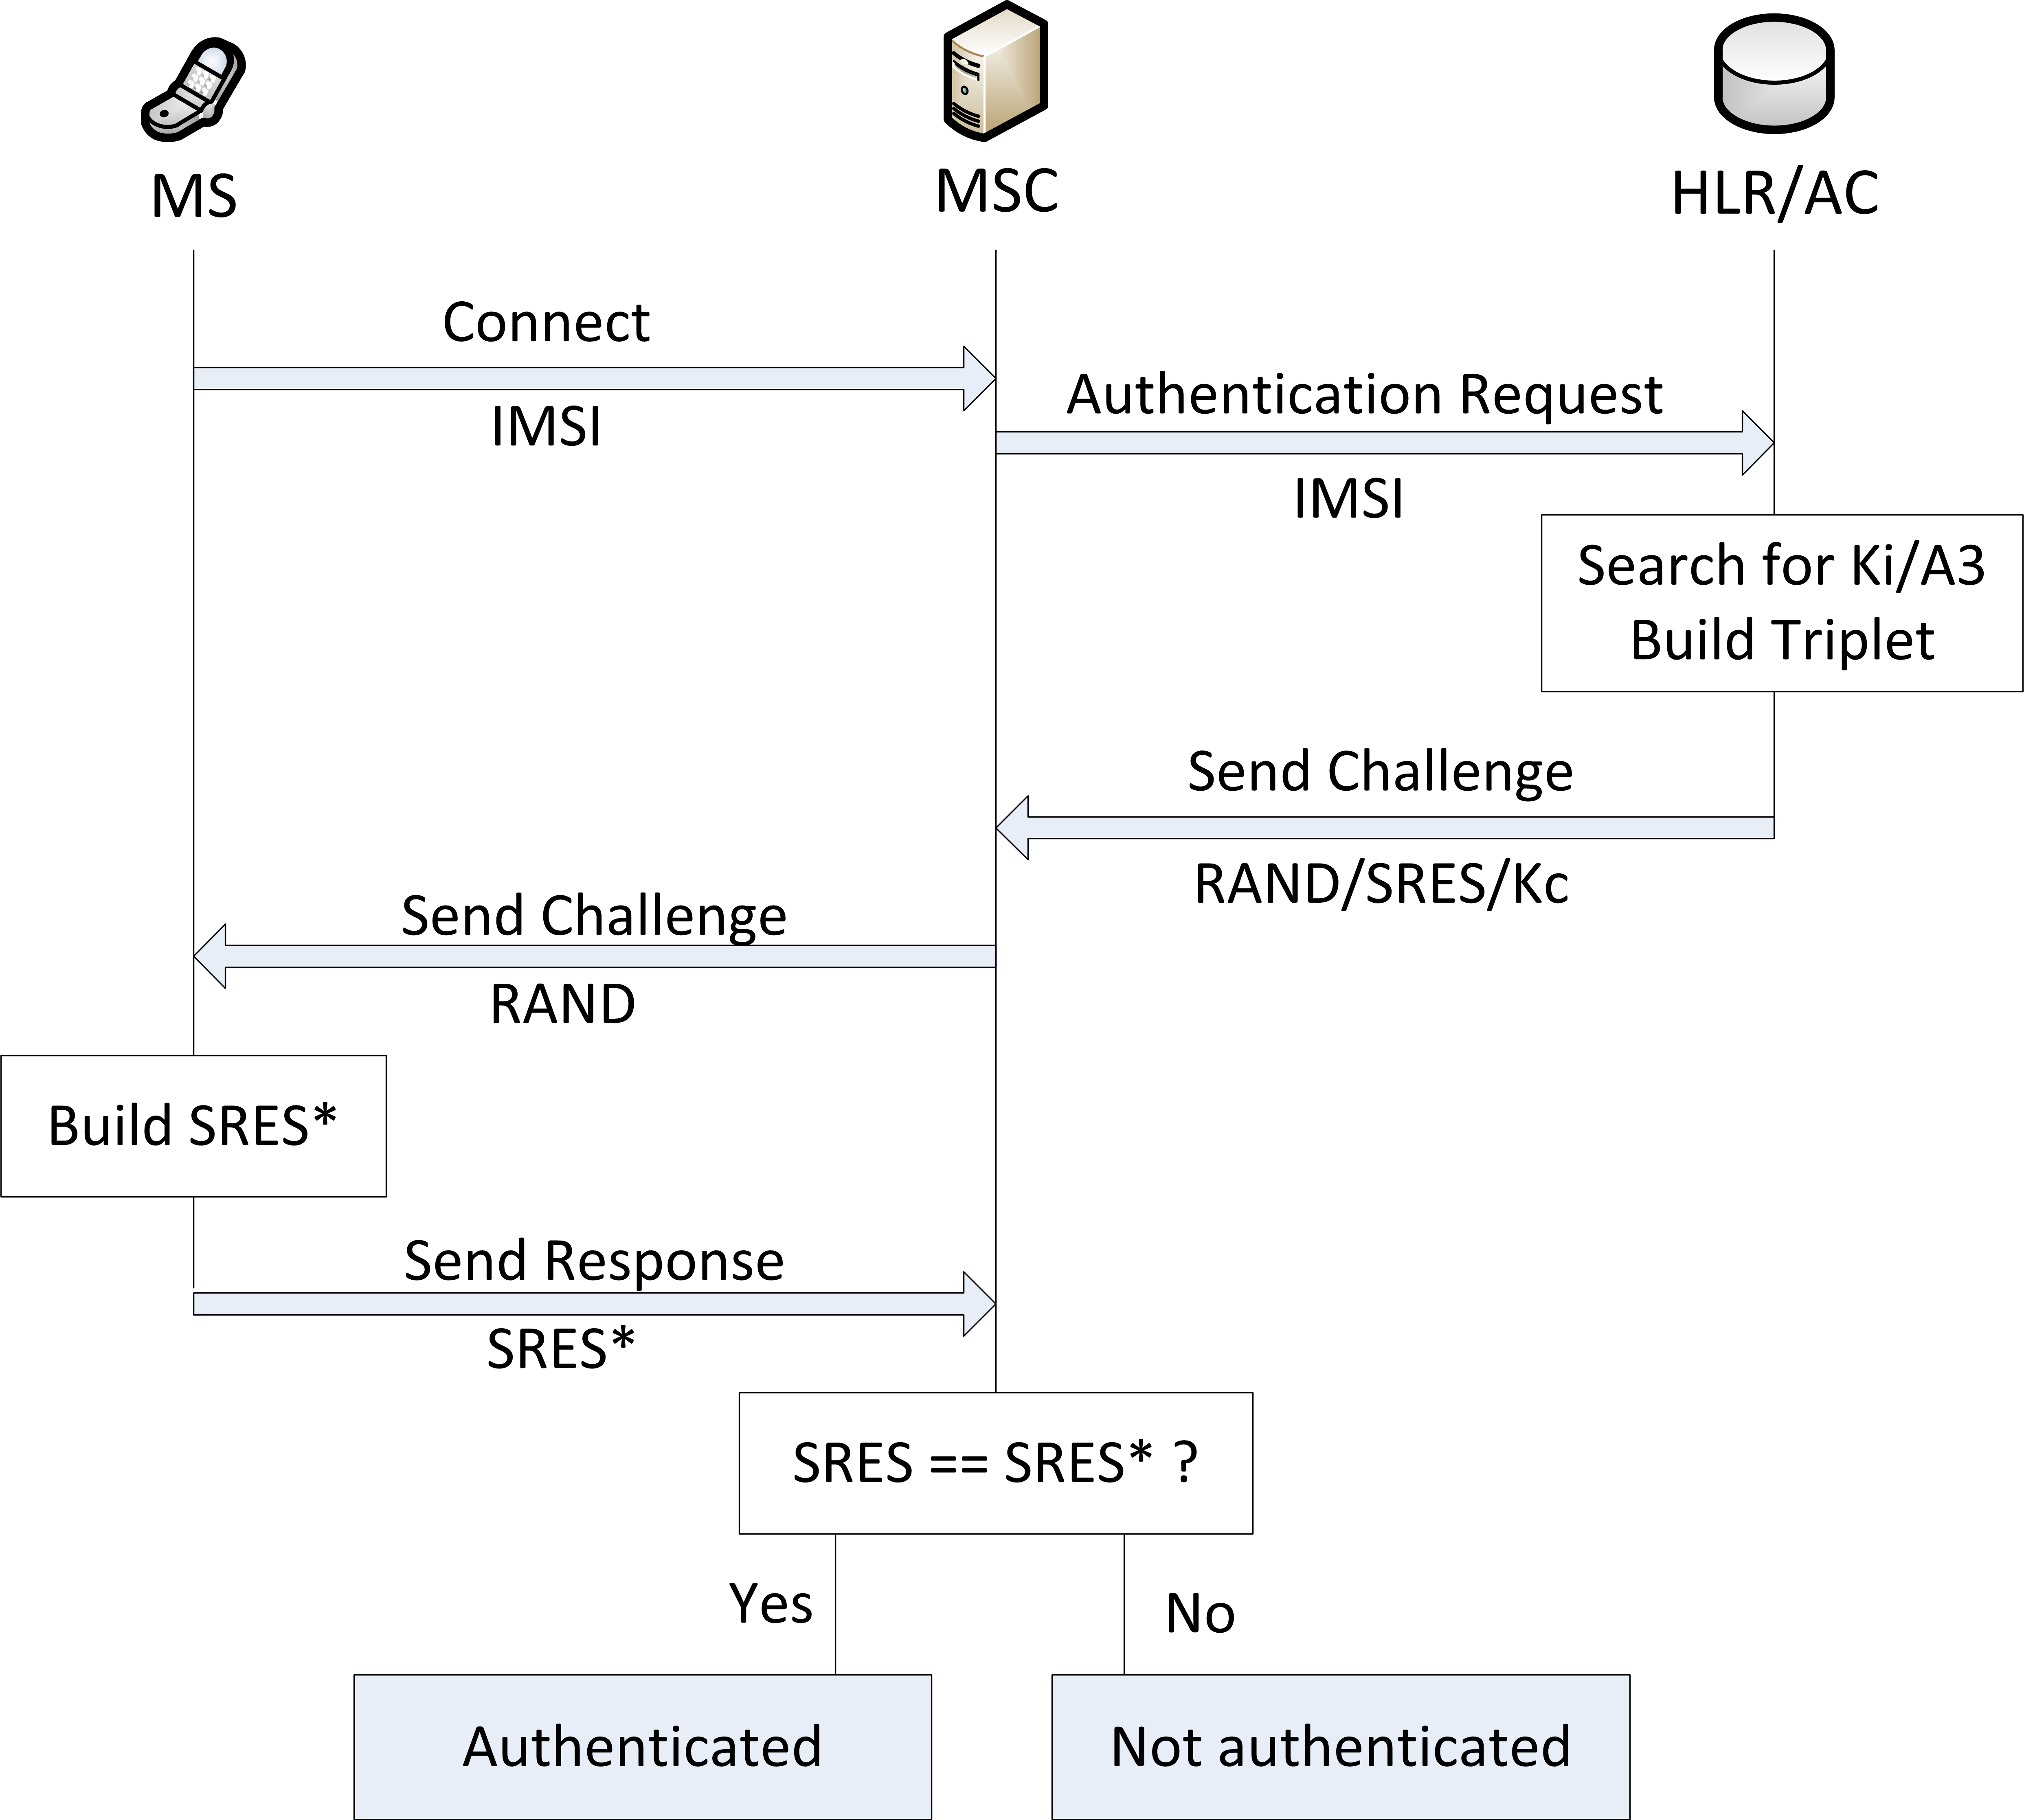
\includegraphics{../Images/Authentication}
\caption{Authentication procedure.}
\label{fig:authentication}
\end{figure}

\subsubsection{Authentication Center}
\label{sec:authentication}
The \gls{ac} is the network component responsible for authenticating mobile subscribers.
It is a part of the \gls{hlr} and the only place apart form the customer's \gls{sim} card where the secret key \gls{ki} is stored.
The authentication is not only done once when the subscriber connects to the network but rather on many occasions \eg the start of a call or other significant events to avoid misuse by a third party.
This authentication routine is a key based challenge-response procedure\footnote{A procedure where a challenge is encrypted with a key only the sender and recipient possess so only the desired person can decrypt the challenge and can send the required response.} outlined in Figure \ref{fig:authentication}.
The steps of the procedure can be summarized as follows:
\begin{enumerate}
	\item User connects to the network or triggers an event that needs authentication at the \gls{msc}.
	There are two possible scenarios from here on.
 	
 	In the first case the \gls{imsi} is part of the authentication request and the \gls{ac} starts with searching for the corresponding \gls{ki} and authentication algorithm A3.
	An authentication triplet is built using \gls{ki} which consists of the components:
	\begin{itemize}
		\item RAND: a 128 bit random number.
		\item SRES: a 32 bit number called signed response, which is generated by A3 with \gls{ki} and RAND as inputs.
		\item Kc: the ciphering key that is used to cypher the data during transmission.
		It is also generated with \gls{ki} and RAND.
	\end{itemize}
	To save signalling bandwidth usually more than one authentication triplet is generated and returned to the \gls{msc} by the \gls{ac}.
	It should be noted that, since a separate cyphering key is used, the secret key never leaves the \gls{ac}.
	
	In the second case either a previously generated authentication triplet is used or new authentication triplets are requested.
	\item RAND is transmitted to the \gls{ms} by the \gls{msc} where the signed response SRES* is created by the \gls{sim} card using A3, \gls{ki} and RAND.
	
	\item An authentication response containing SRES* is sent back to the \gls{msc}.
	
	\item If SRES and SRES* match, the subscriber is authenticated.
\end{enumerate}

Remarkable properties of this procedure are that by using a cyphering key that is generated by a random number and a secret key, the secret key itself never leaves the \gls{ac}.
Apart from that the use of a random number prevents replay attacks on SRES.
It should also be noted that this way of authenticating only works for authenticating the subscriber to the network.
It is a one way authentication.
The subscriber needs to trust the network.
This is a design flaw that IMSI-Catchers use to lure \gls{ms} into their fake network.
In \gls{umts} networks that flaw was fixed and the authentication procedure was made mutual \cite{kommsys2006}.

\subsection{Intelligent Network}
The two subsystems above are necessary for the correct operation of a \gls{gsm} network.
While the \gls{in} is not essential for operation all providers offer additional services that need additional logic and databases.
These databases are called \gls{scp} databases and are one of three possible \gls{ss7} nodes.
They can influence the build-up of a connection or modify parameters for that specific connection.

Two of the most common services offered are \gls{lbs} and prepaid services.
An Example for a well known \gls{lbs} that is provided by the \gls{in} is a dynamic calling rate service.
If the mobile subscriber is in a specific geographical area the \gls{scp} can modify the Billing Record to lower the calling rates.
This is known as home-zone.
If a mobile subscriber uses a prepaid service an account is created for this subscriber that can be topped up.
Afterwards calls and text messaged use up the money on that account.
This is an alternative to a monthly bill and attracted many customers since its advent in the mid 90's.
For this service the \gls{scp} needs to constantly update the money on the account during calls and when text messages are sent.

Since these services were defined as additional and thus no specification existed they evolved into vendor specific proprietary features that were not interoperable.
To standardise these services the \gls{3gpp} and the \gls{etsi} defined the \gls{camel} protocol in TS 23.078 \cite{GSM23078}.
\gls{camel} specifies a protocol much like \gls{http} that regulates how the different components of a \gls{gsm} network exchange information.
As such it is not an application itself but rather a framework to build vendor independent, portable services.

\subsection{Base Station Subsystem}
\label{sec:bss}
The \gls{bss} is the part of the network that provides the hard- and software for physically connecting \glspl{ms} to the provider's network.
Its main components are the \gls{bsc}, the \gls{bts} and the \gls{trau}.
Connecting a mobile subscriber works via radio which is why this subsystem is sometimes also called the radio network \cite{kommsys2006}.
Inside the radio network of a certain area there is one \gls{bsc} that connects to multiple \glspl{bts} and one more \glspl{trau} depending on whether the \gls{trau} is attached to the \gls{bsc} or to all the \glspl{bts}.
While the Transceiver station act as receiver for radio signals the controller coordinates the different receivers and relays the incoming signals  to the core network.
Since signals inside the core network are transmitted at other rates than in the radio network, rates need to be adapted which is done by the \gls{trau}.

Before discussing the individual components of this subsystem it is important to understand how the frequencies of the radio network are used and what architectural impacts this sparse resource has on the network and the components itself.

\subsubsection{Frequencies and the Cellular Principle}
\begin{figure}
\centering
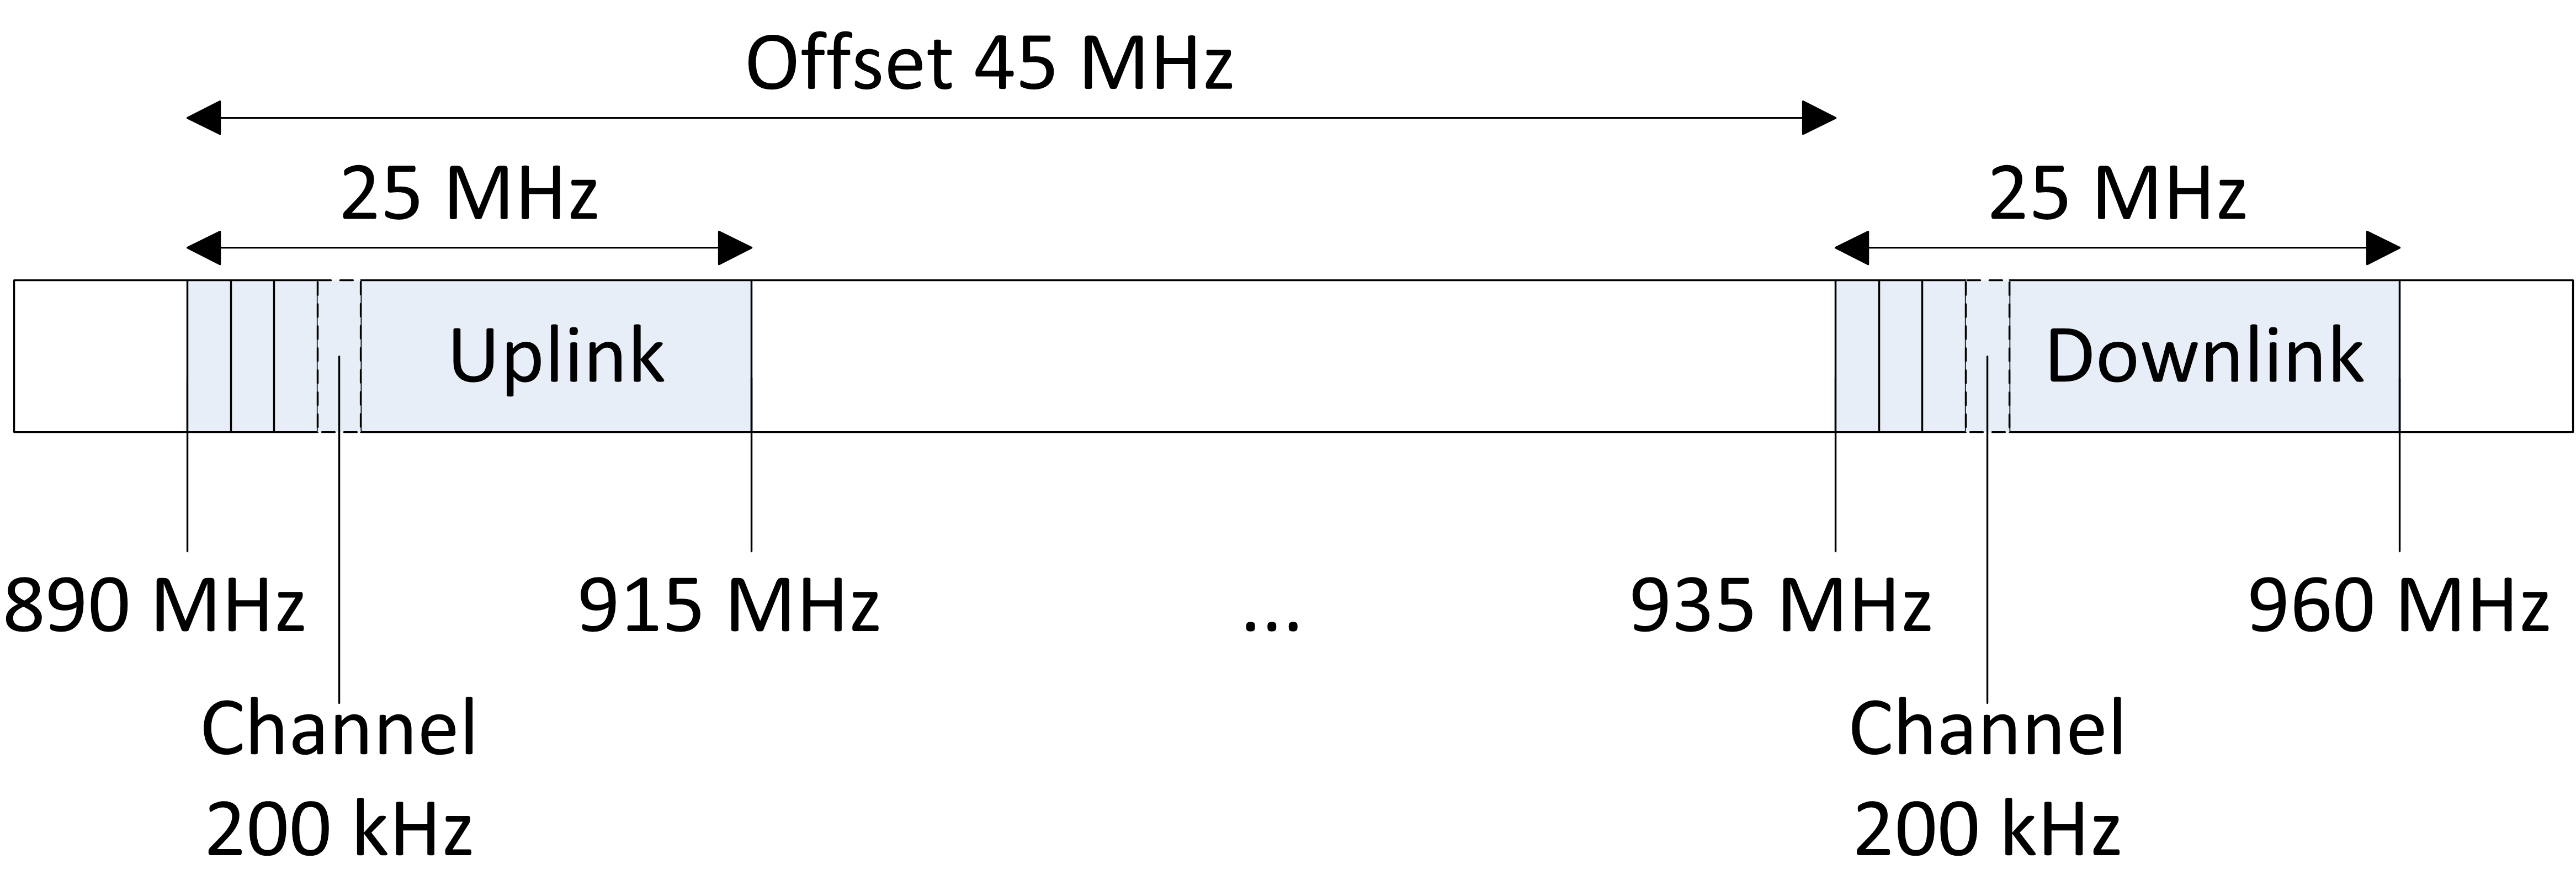
\includegraphics{../Images/Mapping}
\caption{Mapping of functional entities on the 900 Mhz band.}
\label{fig:frequency}
\end{figure}

A frequency band as shown in Figure \ref{fig:frequency} is distributed into different functional entities.
The band is divided into a range for the uplink, the part that is used by the \gls{ms} to upload data into the network and the downlink, that is utilised by the network to send data back.
In the 900 MHz band each of these has a width of 25 MHz.
These bands themselves are furthermore divided into channels, each spanning 200 kHz, which accounts for 125 channels on 25 MHz.

\begin{table}
\centering
\begin{tabular}{lllll}
\toprule
Band		&ARFCN		&Uplink (MHz)	&Downlink (MHz)	&Offset (MHz)\\
\midrule
GSM 900		&0-124		&890-915		&935-960		&45\\
(Primary)	&			&				&				&\\
GSM 900		&0-124		&880-915		&925-960		&45\\
(Extended)	&975-1023	&				&				&\\
GSM 1800	&512-885	&1710-1785		&1805-1880		&95\\
GSM 1900	&512-810	&1850-1910		&1930-1990		&80\\
(North America)	&			&				&				&\\
GSM 850		&128-251	&824-849		&869-894		&45\\
(North America)	&			&				&				&\\
\bottomrule
\end{tabular}
\caption{Frequencies in the different bands \cite{kommsys2006}.}
\label{tab:frequencies}
\end{table}

Each of which is identified by its \gls{arfcn}.
This is a simple numbering scheme, given to those 200 kHz channels.
The frequencies and \glspl{arfcn} are connected as follows:
\begin{align}
F_\text{Uplink} 	&= \text{Start}_\text{Band} + 0.2 \cdot (\text{ARFCN} -(\text{Start}_\text{ARFCN} -1))\\
F_\text{Downlink}   &= F_\text{Uplink} + \text{Offset}_\text{Band}
\end{align}
In case of the 900 MHz Band this would be:
\begin{align}
F_\text{Uplink}		&=890 + 0.2 \cdot (\text{ARFCN} - (1-1))\\
					&=890 + 0.2 \cdot \text{ARFCN}\\
F_\text{Downlink}	&=F_\text{Uplink} + 45
\end{align}

For other bands the numbers differ and can be seen in Table \ref{tab:frequencies} along with their respective \gls{arfcn} numbers but the functionality is the same.

An additional method called time multiplexing which will be explained in further detail in Section \ref{sec:Um}, makes is possible to map $125 \cdot 8 = 1000$ channels that could be used for voice transmission over that band.
Some of these channels need to be used for signalling.
Even though the number by itself seems high it would never suffice to service a large urban area.
This is one of the reasons why another frequency band in the 1800 MHz range has been opened with 75 MHz up- and downlink supporting 375 channels.
That by itself would also never suffice to service the huge number of subscribers therefore the GSM network like any other modern mobile radio network is based on a cellular architecture which makes it possible to reuse frequencies.
The range of one receiver station is drastically reduced to service only a small area.
This is called the cell of the \gls{bts} which in theory can be approximated by a hexagon.
Each of these cells is assigned a different frequency to avoid interference.
However after a certain distance, the frequency reuse distance $D$, is covered the exact same frequency can be used again by another \gls{bts}.
$D$ is chosen large enough so that interference doesn't have an impact on overall call quality.
Figure \ref{fig:cells} shows such an arrangement.
Also a comparison with realistic cells can be seen which differ in their appearance from the optimized hexagon model.
The borders are blurred because of interference, reflection- and shadowing effects and cells in the more urban areas are smaller than cells on the countryside, where the density of subscribers is less and thus can be handled by fewer \glspl{bts}.
The band has been divided into seven frequencies which are only reused (cells with the same number) after distance $D$ is covered.
For an arbitrary division of the frequency band into $k$ partitions and a cell radius of $R$ geometric derivations from the hexagon model yield for the frequency reuse distance $D$ \cite{GSM2009}:
\begin{align}
D	&=R\cdot\sqrt{3k}
\end{align}

This procedure raises the number of effectively usable by a large factor.
However certain disadvantages come with this procedure as well \cite{protocols1999}.
Increasing the amount of receivers automatically increases the cost of infrastructure for the provider.
Due to the nature of the mobility of subscribers this increases the amount of Handovers needed since it is more likely that a subscriber leaves a small cell during an active call.
Also an update of the location of a subscribers needs to be done more often to ensure reachability for incoming calls.
These inflict increased signalling load on the network itself.

\begin{figure}
\centering
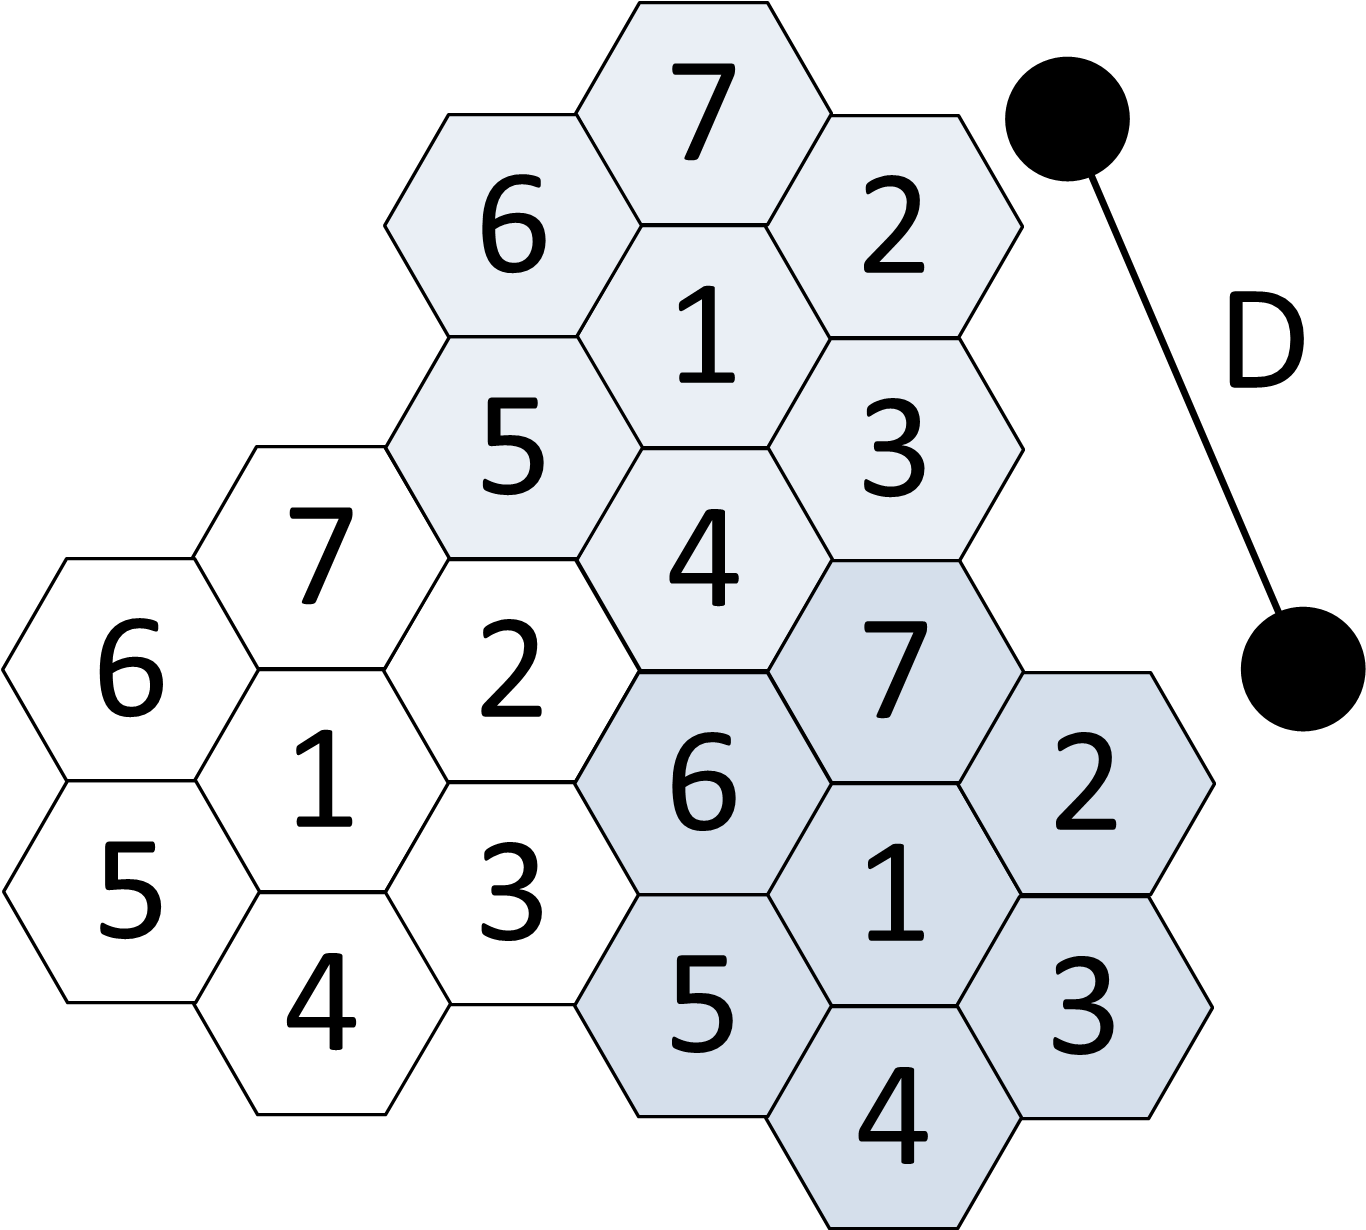
\includegraphics{../Images/Cells}
\hspace{1cm}
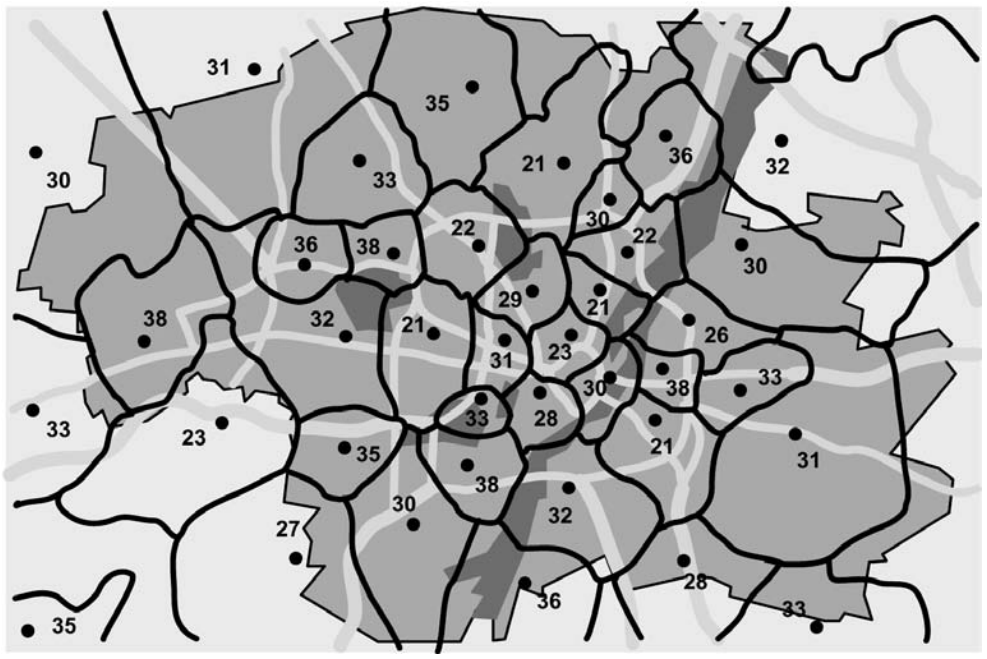
\includegraphics[scale=.21]{../Images/real_Cells}
\caption{Theoretical arrangement of radio cells compared to a realistic alignment. Cells with the same number share the same frequency \cite{GSM2009}.}
\label{fig:cells}
\end{figure}

\subsubsection{Base Transceiver Station}
They are also called Base Stations and are the entry points to the network for subscribers.
Theoretically a \gls{bts} can serve a cell of 35 km radius however this is decreased by interference, reflection- and shadowing effects.
The limiting factor here are the number of subscribers itself.
A single station can only serve a limited number of users which yields a radius as low as 100 m for a single \gls{bts} in dense urban housing areas \cite{kommsys2006}.
On the countryside where population is less dense the constraining factor can also be transmission power of the \gls{me}.
Therefore cells with a radius above 15 km are seldom seen.

\begin{figure}
	\centering
	\subfigure[Stantard configuration.]{\centering\includegraphics{../Images/standart_config}}
	\subfigure[Umbrella cell configuration.]{\centering\hspace{1cm}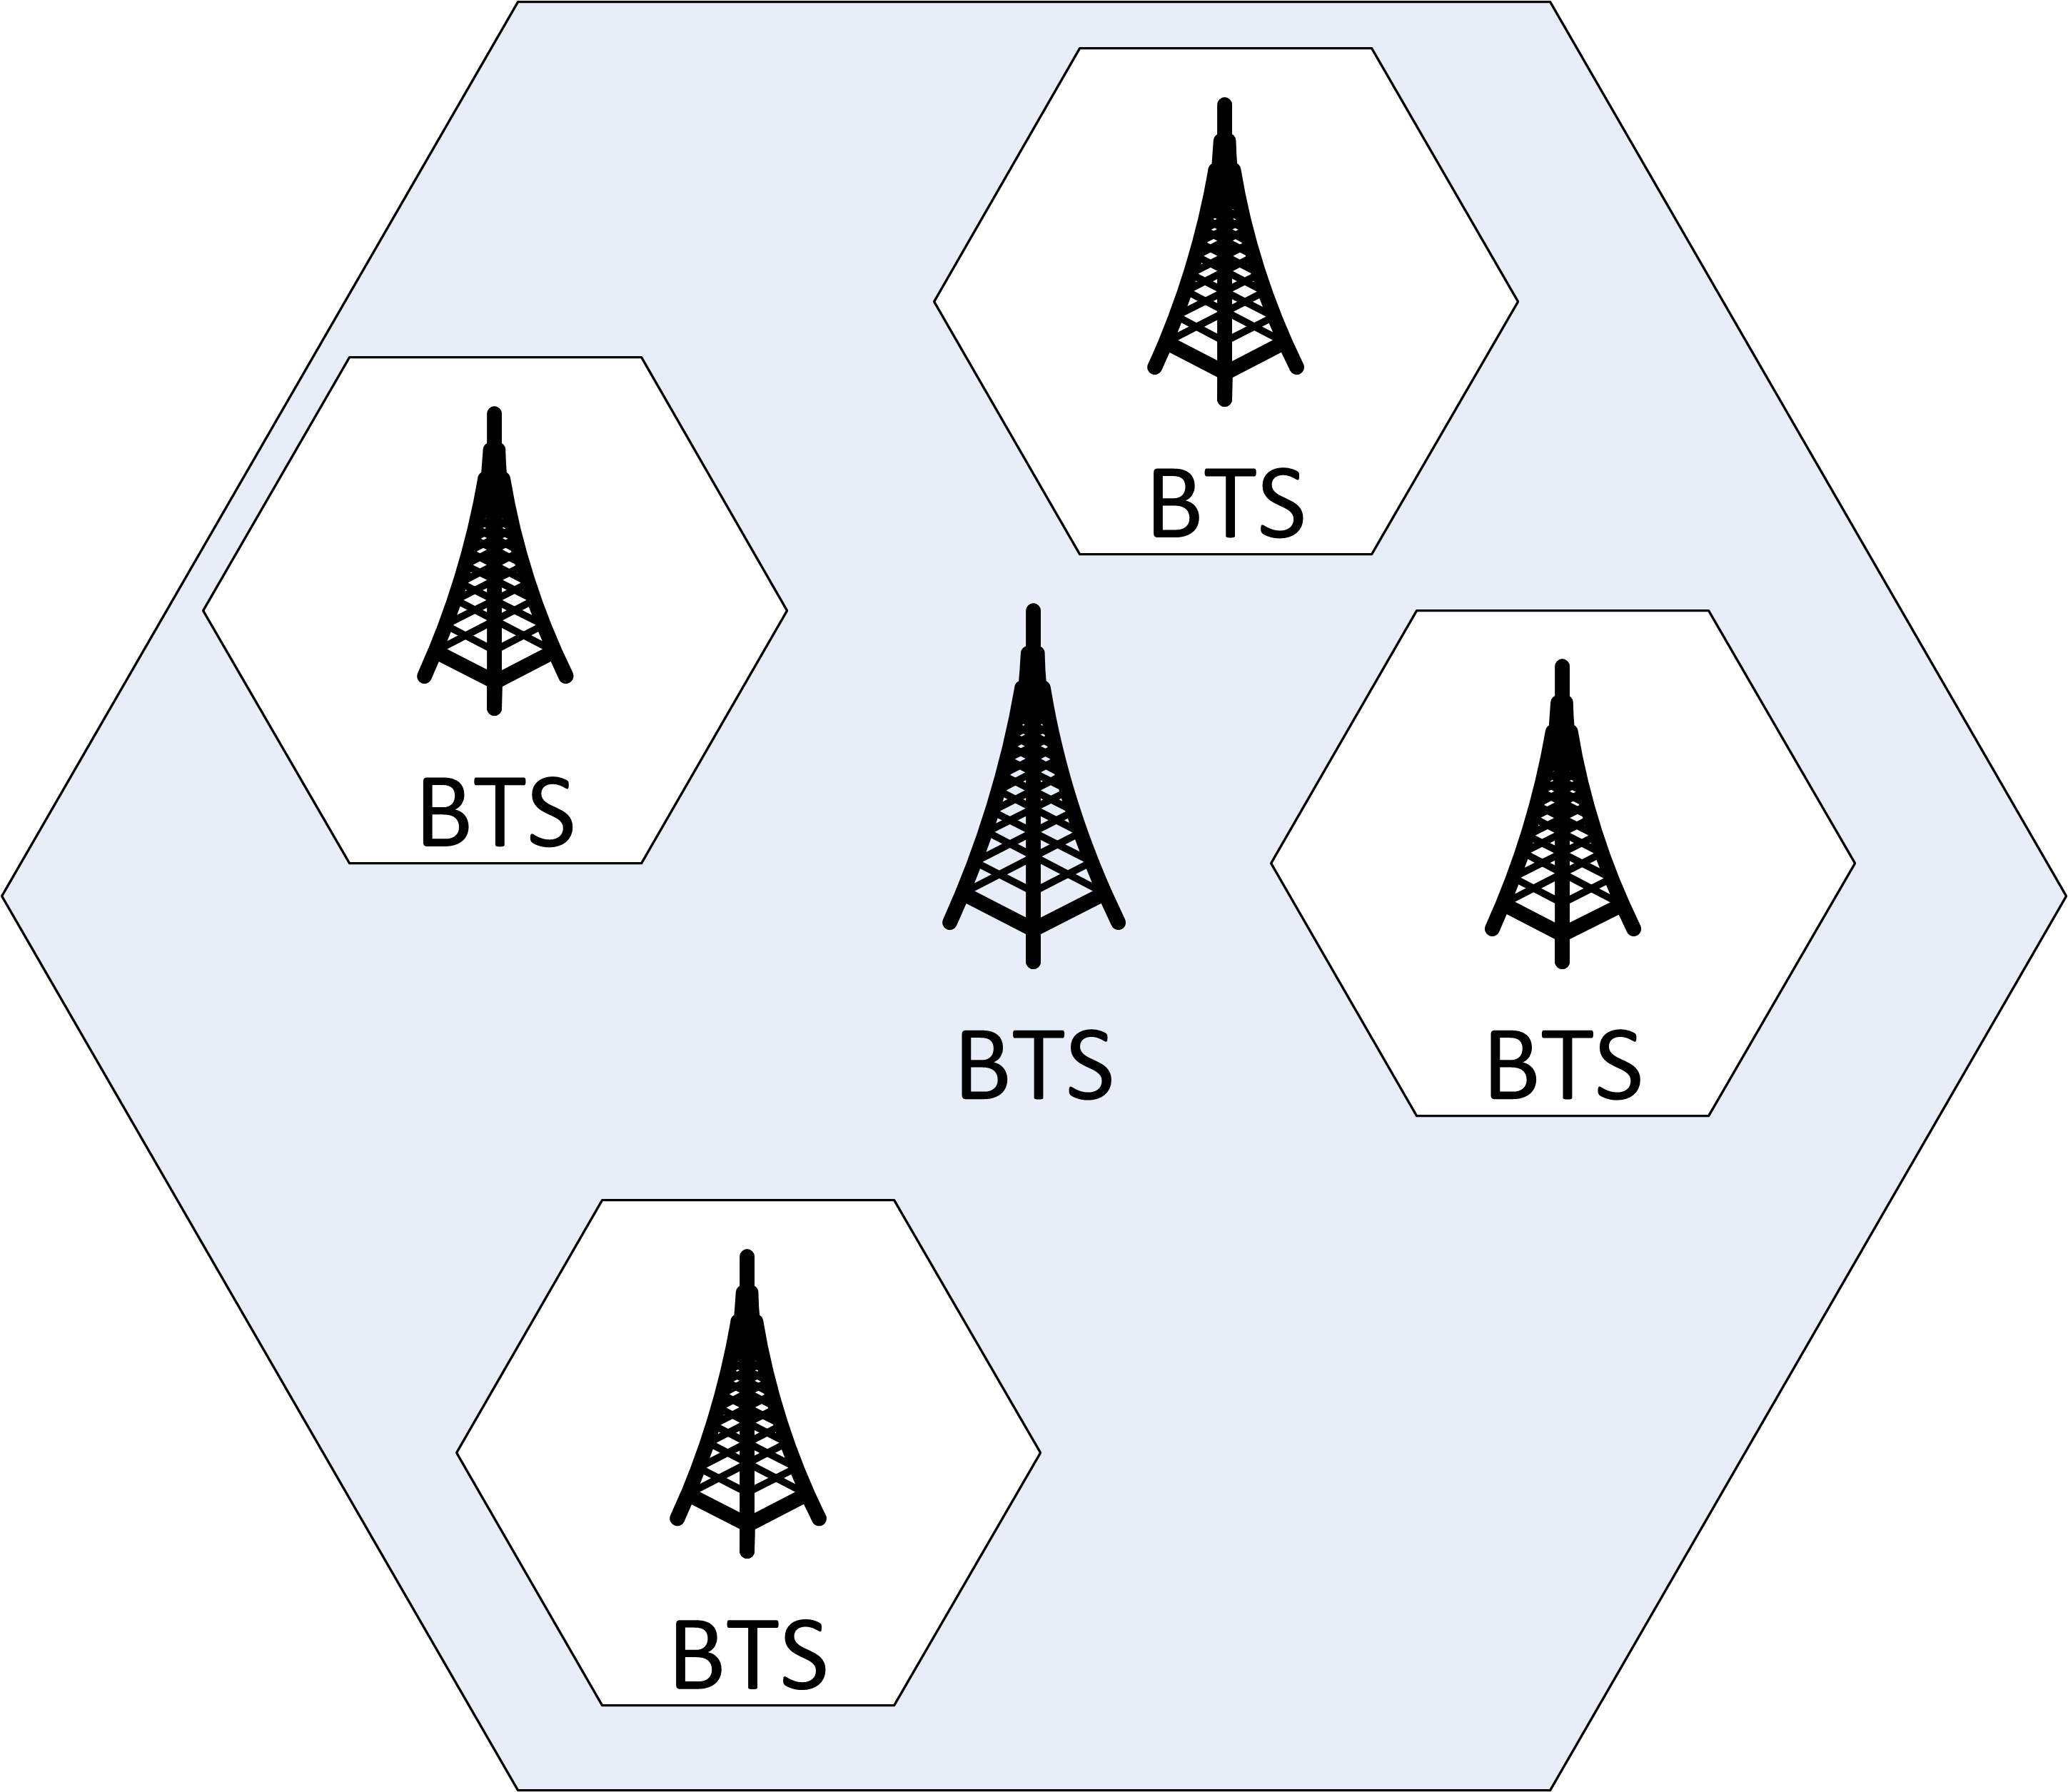
\includegraphics{../Images/Umbrella}\hspace{1cm}}
	\subfigure[Sectorised configuration.]{\centering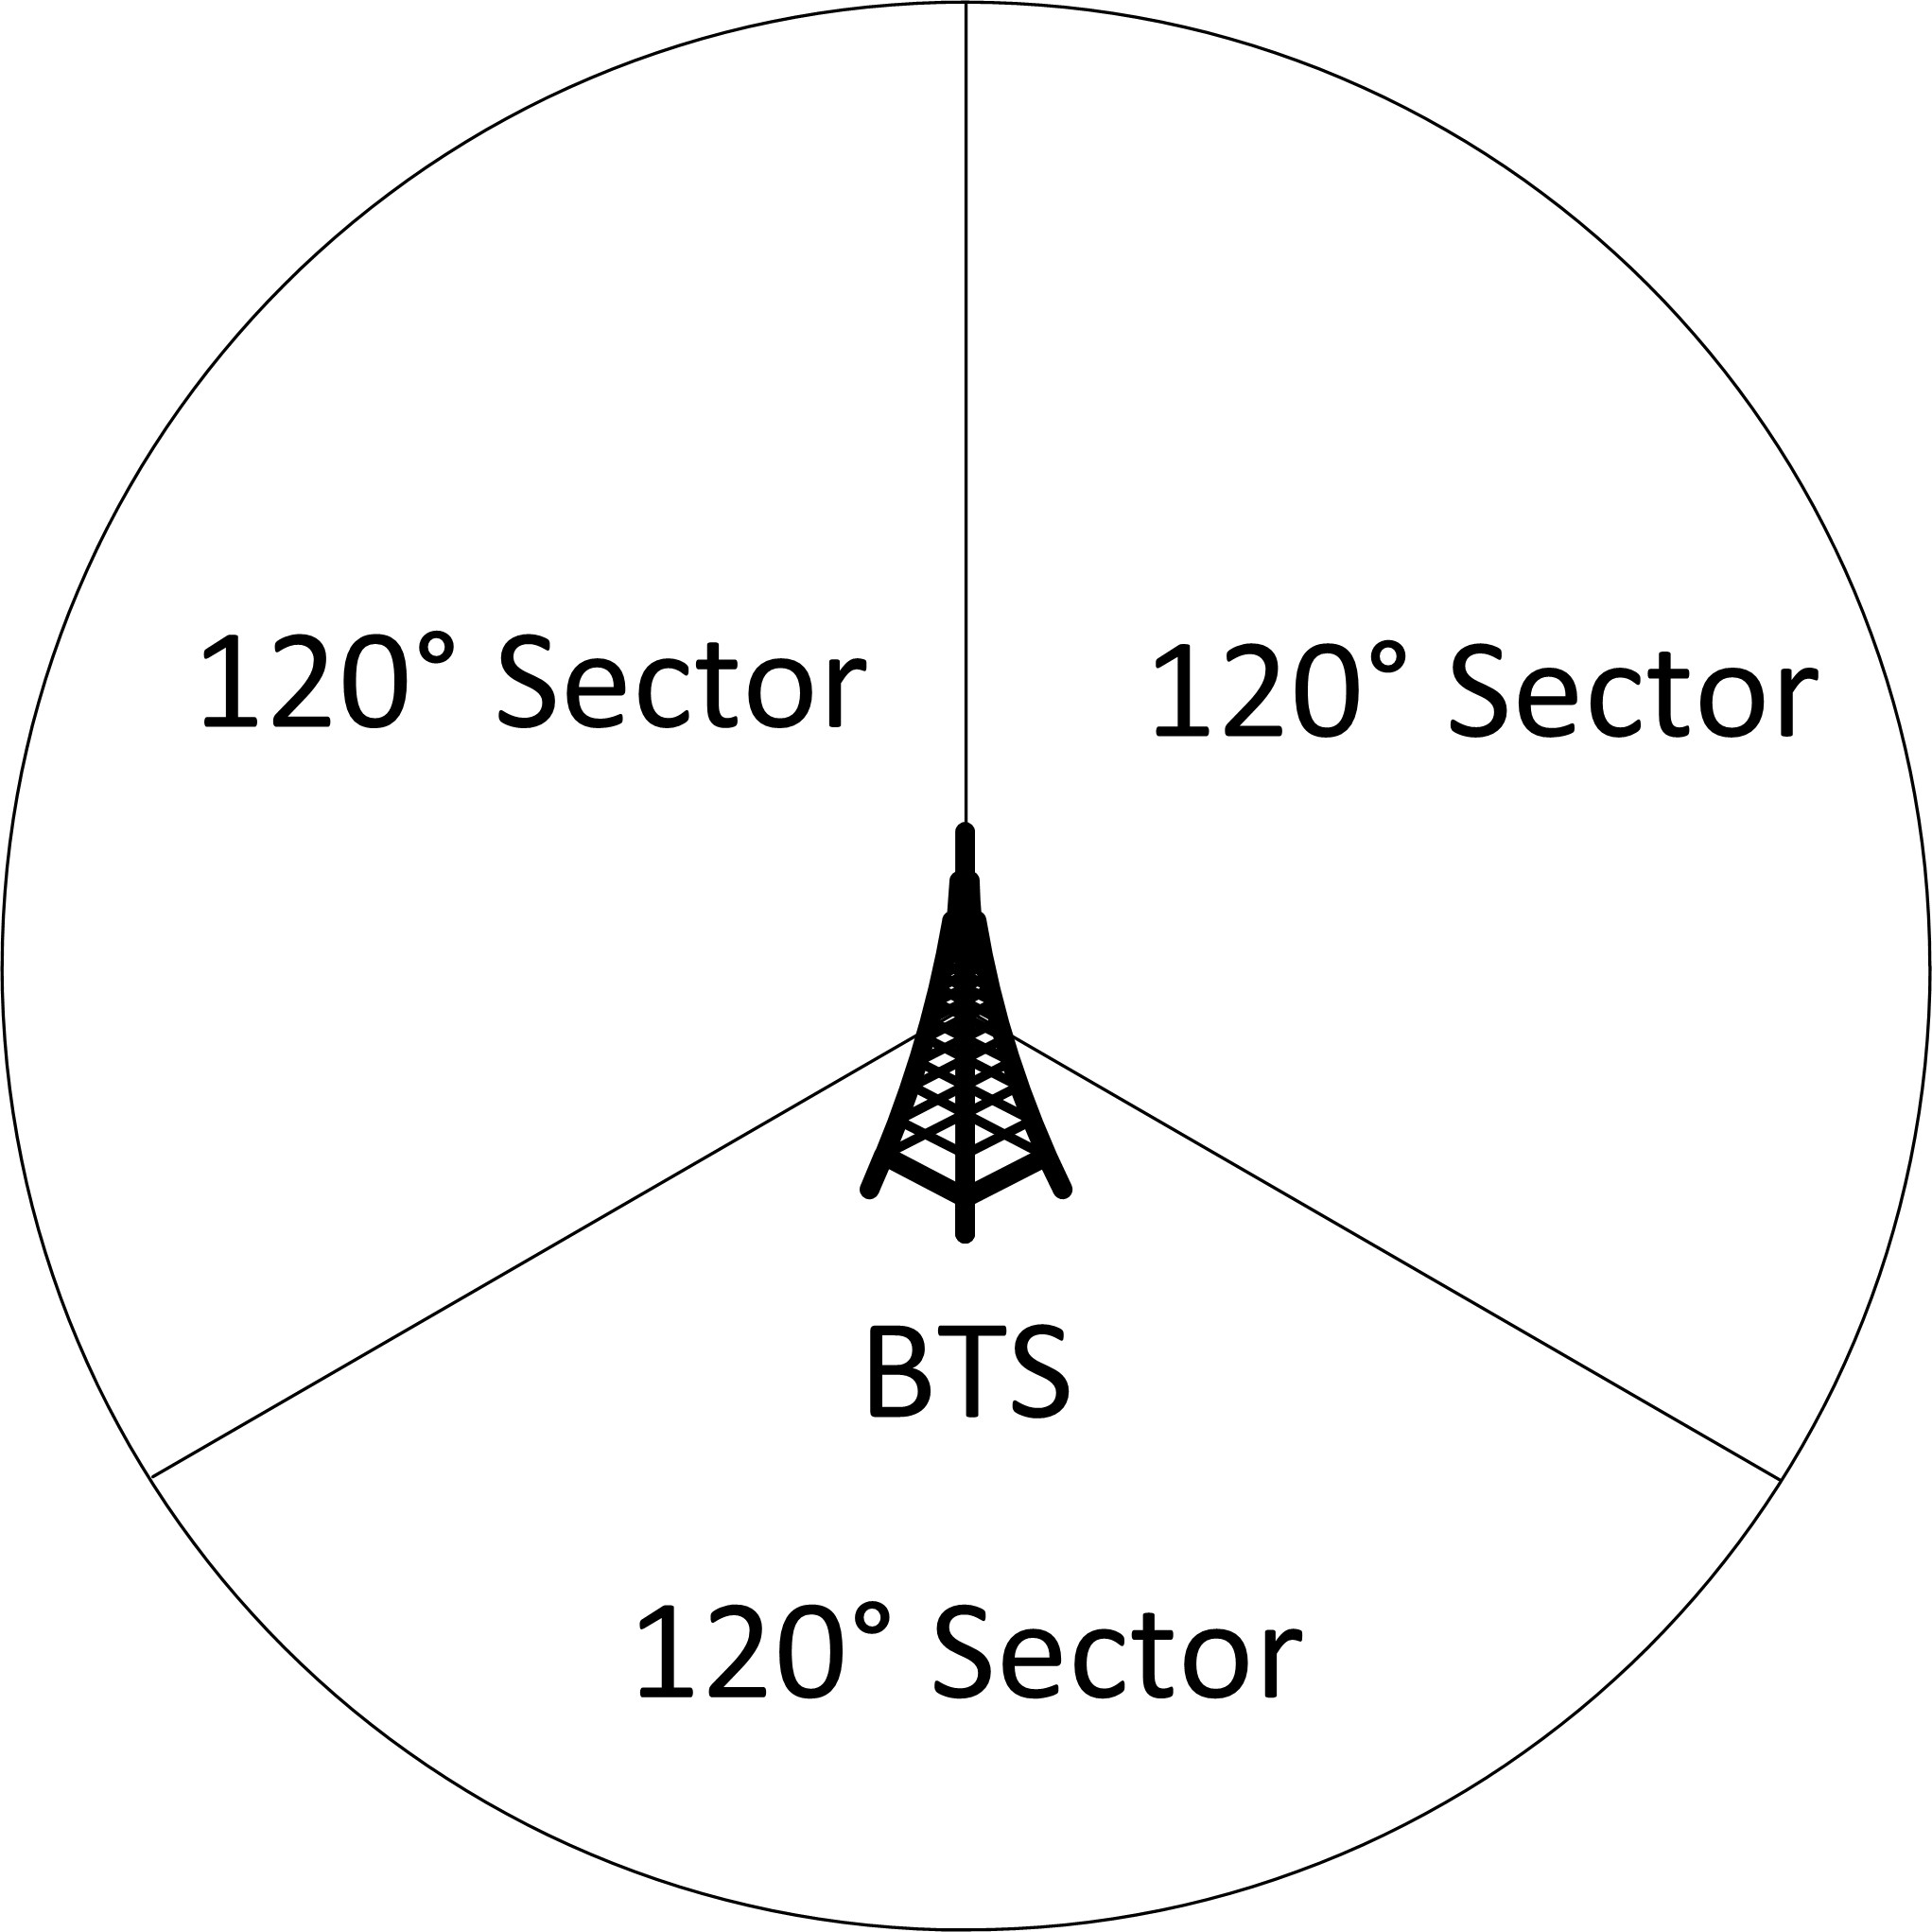
\includegraphics{../Images/Sectorised}}
	\caption{Common base station configurations. Compiled from \cite{protocols1999}.}
	\label{fig:configurations}
\end{figure}

\glspl{bts} and their corresponding cells can have different configurations depending on load or morph structure of the surroundings.
The main configurations will now be discussed shortly.

In a \emph{standard configuration} every base base station has its own \gls{ci}, it is a one to one mapping of cells to \gls{bts}.
This is an cost effective way of providing service to a rural or sparse settled area.
An comparative illustration of configurations can be found in Figure \ref{fig:configurations}.

The \emph{umbrella configuration} is build around one central \gls{bts} that is on high ground compared to its neighbours and has a higher transmission power.
Thus the notion of this particular base station wrapping all the others in the area.
Due to interference the frequency used by the wrapping base station cannot be used by the others.
Nevertheless in some scenarios like alongside highways in urban areas this makes sense.
A car that moves fast from one cell to the next may need a lot of Handovers thus inflicting a large amount of signalling load on the network.
These fast moving subscribers are assigned to the umbrella station, that way less to no Handovers are needed.
This configuration however is not defined in the \gls{gsm} specifications and needs additional software in the \gls{bsc} thus it is considered a proprietary function \cite{protocols1999}.

The \emph{sectorised configuration} has become the de facto standard for urban areas.
In the other configurations a single \gls{bts} covers always a 360$^\circ$ area, and a certain distance is kept to its next neighbour to avoid interference in overlapping areas.
The idea is to use antennas which only cover a certain angle, like 180$^\circ$, 120$^\circ$ or 60$^\circ$ dividing a cell into two, three or six sectors respectively each having its own \gls{bts}.
Main advantages are that each single \gls{bts} has to deal with less subscribers and that in a multi-sector configuration frequencies can be reused inside a cell, which is  a great advantage for these densely settled areas.

\subsubsection{Baste Station Controller}
The \gls{bsc} is the central unit in the \gls{bss}.
It can be compared to a digital exchange in a standard telephone network with additional mobile extensions.
The design idea was to remove all radio related load from the \gls{msc} into the radio subsystem.
Therefore a \gls{bsc} manages the multitude of \glspl{bts} in the \gls{bss}.

First and foremost it is a switching centre.
This means it has to switch incoming traffic channels from the \gls{msc} over the A-interface to channels on the outgoing A$_\text{bis}$-interface which leads over the \gls{bts} and thus the air interface to different \glspl{ms}.
As a result the initialisation and maintenance of signalling and voice channels are its main tasks.
What channels are and how they are established is explained in Section \ref{sec:channels}.
For the sake of functional explanation of the \gls{bsc} it will suffice to regard channels as a communication line for a particular purpose like receiving or sending voice data or  for sending broadcast information.
Due to the nature of a mobile network certain other tasks have to be performed like Handovers and power management \cite{kommsys2006}.
We will now look at the different tasks in more detail.

A \emph{signalling channel} is needed when a subscriber wants to start a call or send a text message.
The \gls{ms} sends a channel request message to the \gls{bsc} which needs to check if any \glspl{sdcch} are free.
If there are free channels, one of those channels is activated via the \gls{bts} and an immediate assignment message is sent via the \gls{agch} containing the number of the assigned channel.
From this point on the \gls{ms} can sent data on the assigned channel that reach the \gls{msc}.
For incoming calls a prior step has to be taken.
The \gls{msc} sends a message to the \gls{bsc} that contains the \gls{imsi}, \gls{tmsi} and \gls{la} of the subscriber that is being called or texted.
This message is forwarded to and broadcasted by all cells in that \gls{la} on the \gls{pch}.
As soon as this message arrives at the respective \gls{ms} it requests a channel with the procedure outlined above.

After a signalling channel is found that way, a \emph{voice channel} can be initialised.
The \gls{msc} sends an assignment request message to the \gls{bsc} after the start of the call has been determined on the previously assigned \gls{sdcch} between the \gls{msc} and the \gls{ms}.
A free \gls{tch} is assigned and the \gls{ms} can tune in to this channel and send an acknowledgement to the \gls{bsc}, which in turn sends an acknowledgement that the assignment has been completed to the \gls{ms} and the \gls{msc}.

\emph{Power management} is an essential part for heightened mobility.
Basis for power management is that continuous measurements have to be done.
These signal quality measurements are taken by the \gls{bts} and forwarded to the \gls{bsc}.
Whenever transmission strength has to be turned up or can be turned down, the \gls{bsc} informs the \gls{bts} which in turn distributes the information periodically to the connected mobile phones via a \gls{sacch}.
Minimisation of transmission power has the advantage of longer uptime for \glspl{ms} since the battery will be less strained.

As mentioned before a \emph{Handover} is necessary when a subscriber leaves the area of a cell and needs to be assigned to another one or if the reception of the current cell at the subscriber's end is far worse than those of neighbouring cells.
A Handover takes place during an active call therefore first of all a \gls{tch} in the target cell has to be activated.
Once this is done the new cell address and frequency is sent to the \gls{ms} over the \gls{facch} along with a command that triggers the Handover.
After synchronising with the new cell an acknowledgement is sent by the base station to the controller to switch the voice connection to the new cell.
What remains is freeing the old \gls{tch} for further use by other subscribers.

\subsubsection{Transcoding rate and Adaption Unit}
Inside the \gls{nss} voice data is moved with 64 kBit/s over E-1 connections.
The resources on the air interface are much scarcer, therefore this amount of voice data cannot directly be sent to \glspl{ms} through the radio network.
The data rate on the $U_m$ interface for voice is about 22.8 kBit/s as will be broken down in detail in Section \ref{sec:radio}.
Since the channel is noisy and prone to errors, a lot of this bandwidth has to be subtracted for error correction purpose leaving around 13 kBit/s for actual voice data \cite{kommsys2006}.
The 64 kBit/s PCM signal is sent from the \gls{msc} to the \gls{ms}, on its way it is compressed and then sent over the air interface.
On the other side, the compressed 13 kbit/s signal is decompressed to 64 kBit/s again.
The compression and decompression on the subscriber's side is handled by the \gls{me} while on the network side the \gls{trau} is responsible for these tasks.
Additionally the \gls{trau} can choose from a variety of codecs (compression/decompression algorithms).
The one normally used is called Full Rate codec.
Another codec is the Half Rate codec which compresses the voice signal to 7 kBit/s thus making it possible to double the amount of \glspl{tch} since one channel can be used to transfer two different voice signals.
This is interesting for crowded events where a lot of subscribers need to be served by a relatively small number of \gls{bts}.

One of the most important tasks of the \gls{trau} apart from compressing, decompressing and correcting transmission errors is ciphering the voice data.
As in most cases when handling continuous data a stream cyphering algorithm is used.
The stream cypher key $K_c$ that is generated by the authentication centre.
It is generated by the A8 algorithm on the \gls{sim} card with a random number (RAND) and the secret key \gls{ki} as input.
Since the transmission of voice data is split into frames it suffices to encode the data on a per frame basis.
\gls{kc} and the current frame number are the inputs for the algorithm A5 which generates a 114 bit cyphering sequence that can be XORed with the frame.
This sequence changes every frame since it uses the current frame number as input.
The complete procedure is outlined in Figure \ref{fig:cypher}.

\begin{figure}
\centering
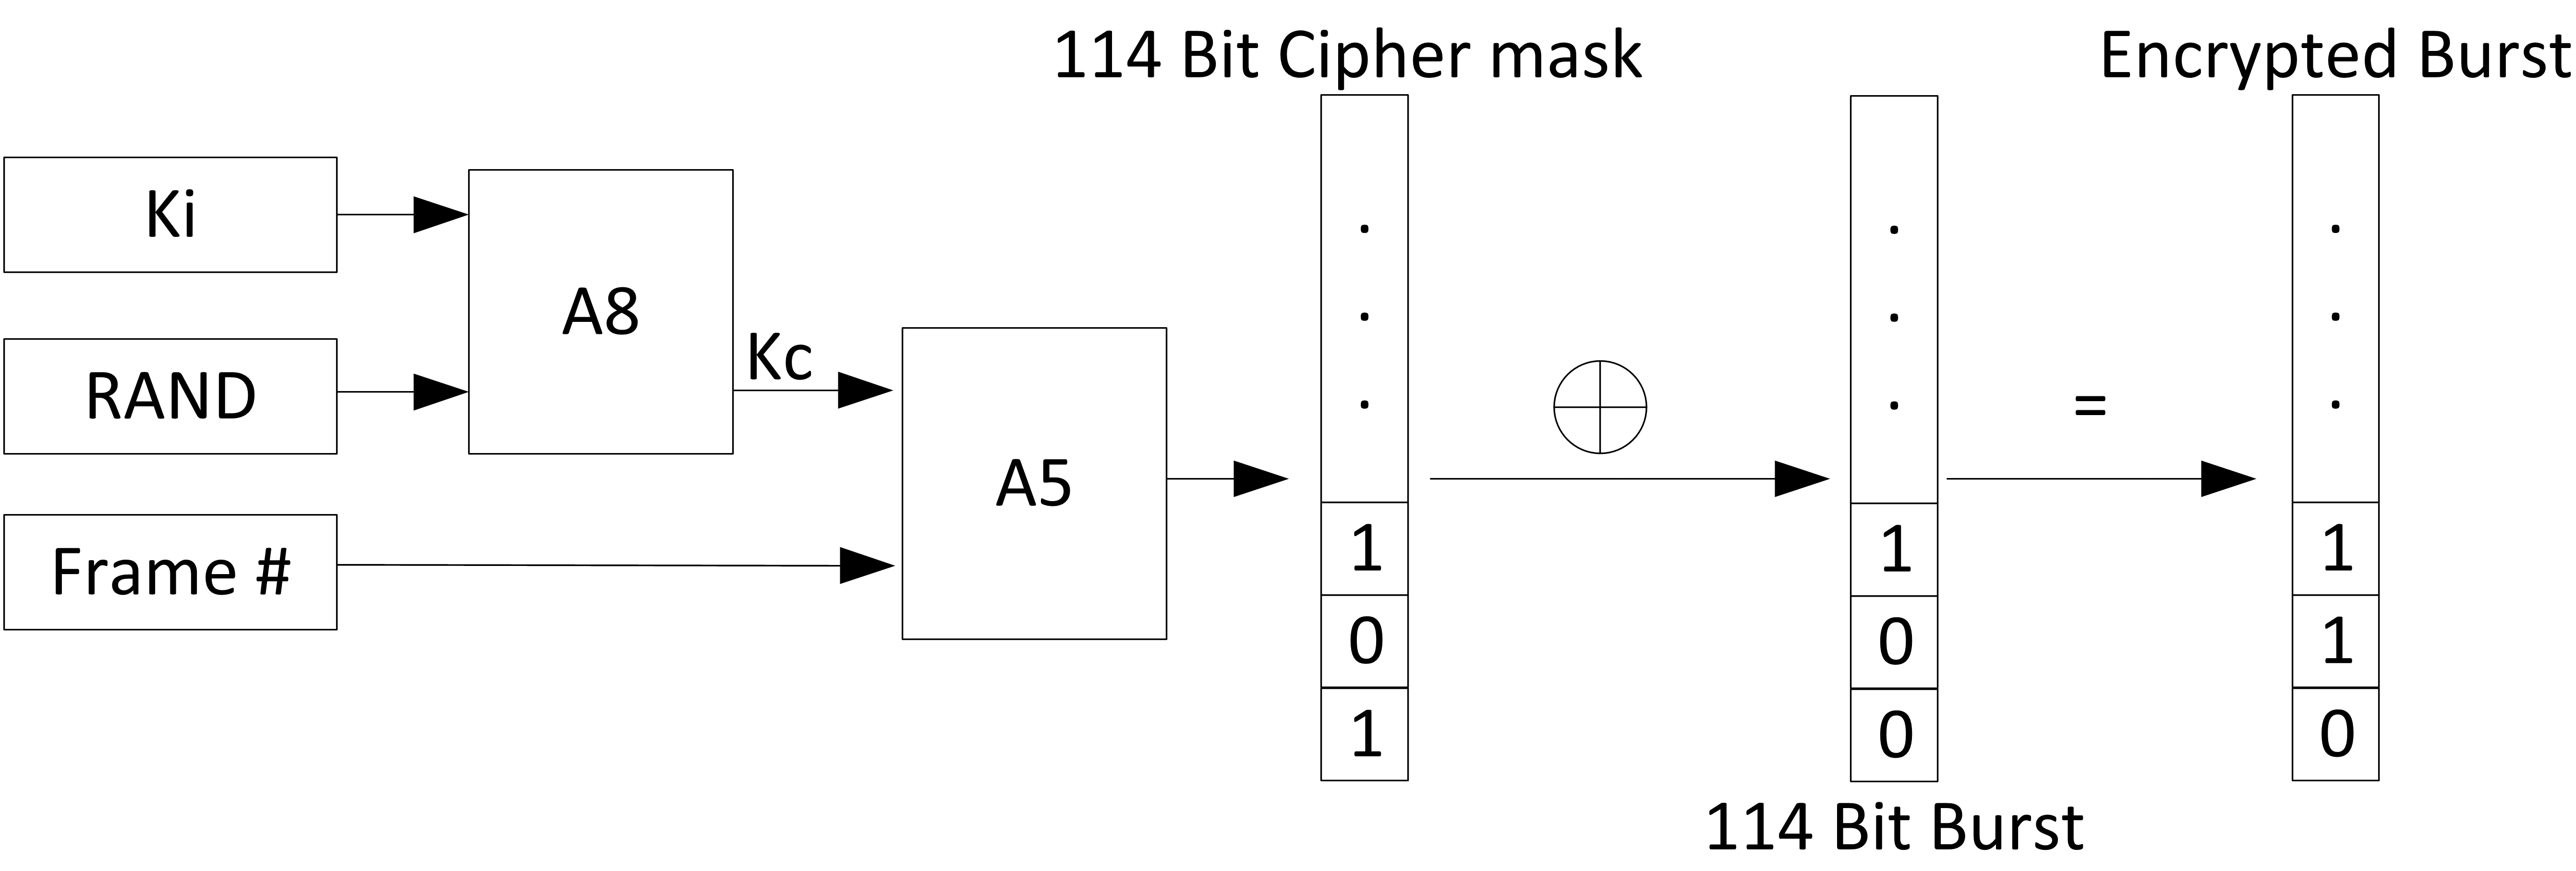
\includegraphics{../Images/Cipher}
\caption{Ciphering procedure for one frame of voice data. Adopted from \cite{kommsys2006}.}
\label{fig:cypher}
\end{figure}

Some strong ciphering algorithms are not permitted in certain countries so there is a variety of algorithms called A5/1, A5/2,$\ldots$ A5/n from which one needs to be chosen upon connecting to the network.
However the encryption in only optional and not mandatory.
If the network does not offer encryption, the \gls{me} sends its data unencrypted, without giving notice to the user in most cases.
The other weakness is the locality of encryption.
The procedure only affects the transmission from the \gls{me} to the \gls{bts}, everything after that is unencrypted voice data.
This is especially a problem when providers use point-to-point radio systems to connect their base stations to the \gls{msc}.

\section{The $U_m$ Interface}
\label{sec:Um}
As with all radio based networks the efficiency of the wireless interface, the interface between the \gls{ms} and the \gls{bts} is of utmost importance to the overall performance of the network.
The main reason for that is that resources on the air interface are scarce.
Efficiency in this case can be seen as maximizing the quotient of transmission rate over bandwidth used \cite{protocols1999}.

The first section will explain how transmission in a \gls{gsm} network is handled on the physical level and what techniques are used to maximize throughput.
Afterwards the notion of logical channels, virtual channels that are mapped on top of the actual transmission, will be discussed and which channels are of importance for this project.
The last section compares the network layers of the \gls{gsm} stack to the ISO/OSI layer model, to give a basis for understanding where the framework employed in the practical part is situated in that hierarchy.

\subsection{Radio Transmission}
\label{sec:radio}
Without additional techniques, the \gls{bts} would only be able to serve a single caller at a time. 
Therefore even in older radio networks like the C-Netz in Germany \gls{fdma} is used.
With \gls{fdma} a specific frequency of the broad frequency band of the \gls{bts} is allocated to a specific subscriber for a call, leaving other frequencies open to use for other subscribers connected to the same base station.
Essentially this means that every \gls{bts} can serve multiple frequencies at the same time.
This comes at the cost of additional hardware, since all the frequencies need their own transceivers and need to be amplified accordingly to guarantee the transmission quality.
Additional hardware for each channel is also required to enable duplex transmission, meaning that sending and receiving can be done at the same time.

That number of available frequencies would not suffice to meet the demand, more communication channels were needed.
To that end another technique has been introduced, called \gls{tdma}.
In \gls{gsm} networks each of these sub-bands yielded by the \gls{fdma} procedure has a width of 200 kHz.
Onto this smaller carrier frequency, \gls{tdma} frames are transmitted, that contain eight time slots.
These frames have a transmission length of 4.615 ms.
Each of these timeslots could host the data of a different subscriber, although the first one is usually used for signalling procedures.
An illustration of how these multiplexing methods work together can be seen in Figure \ref{fig:fdma_tdma}.

\begin{figure}
	\centering
	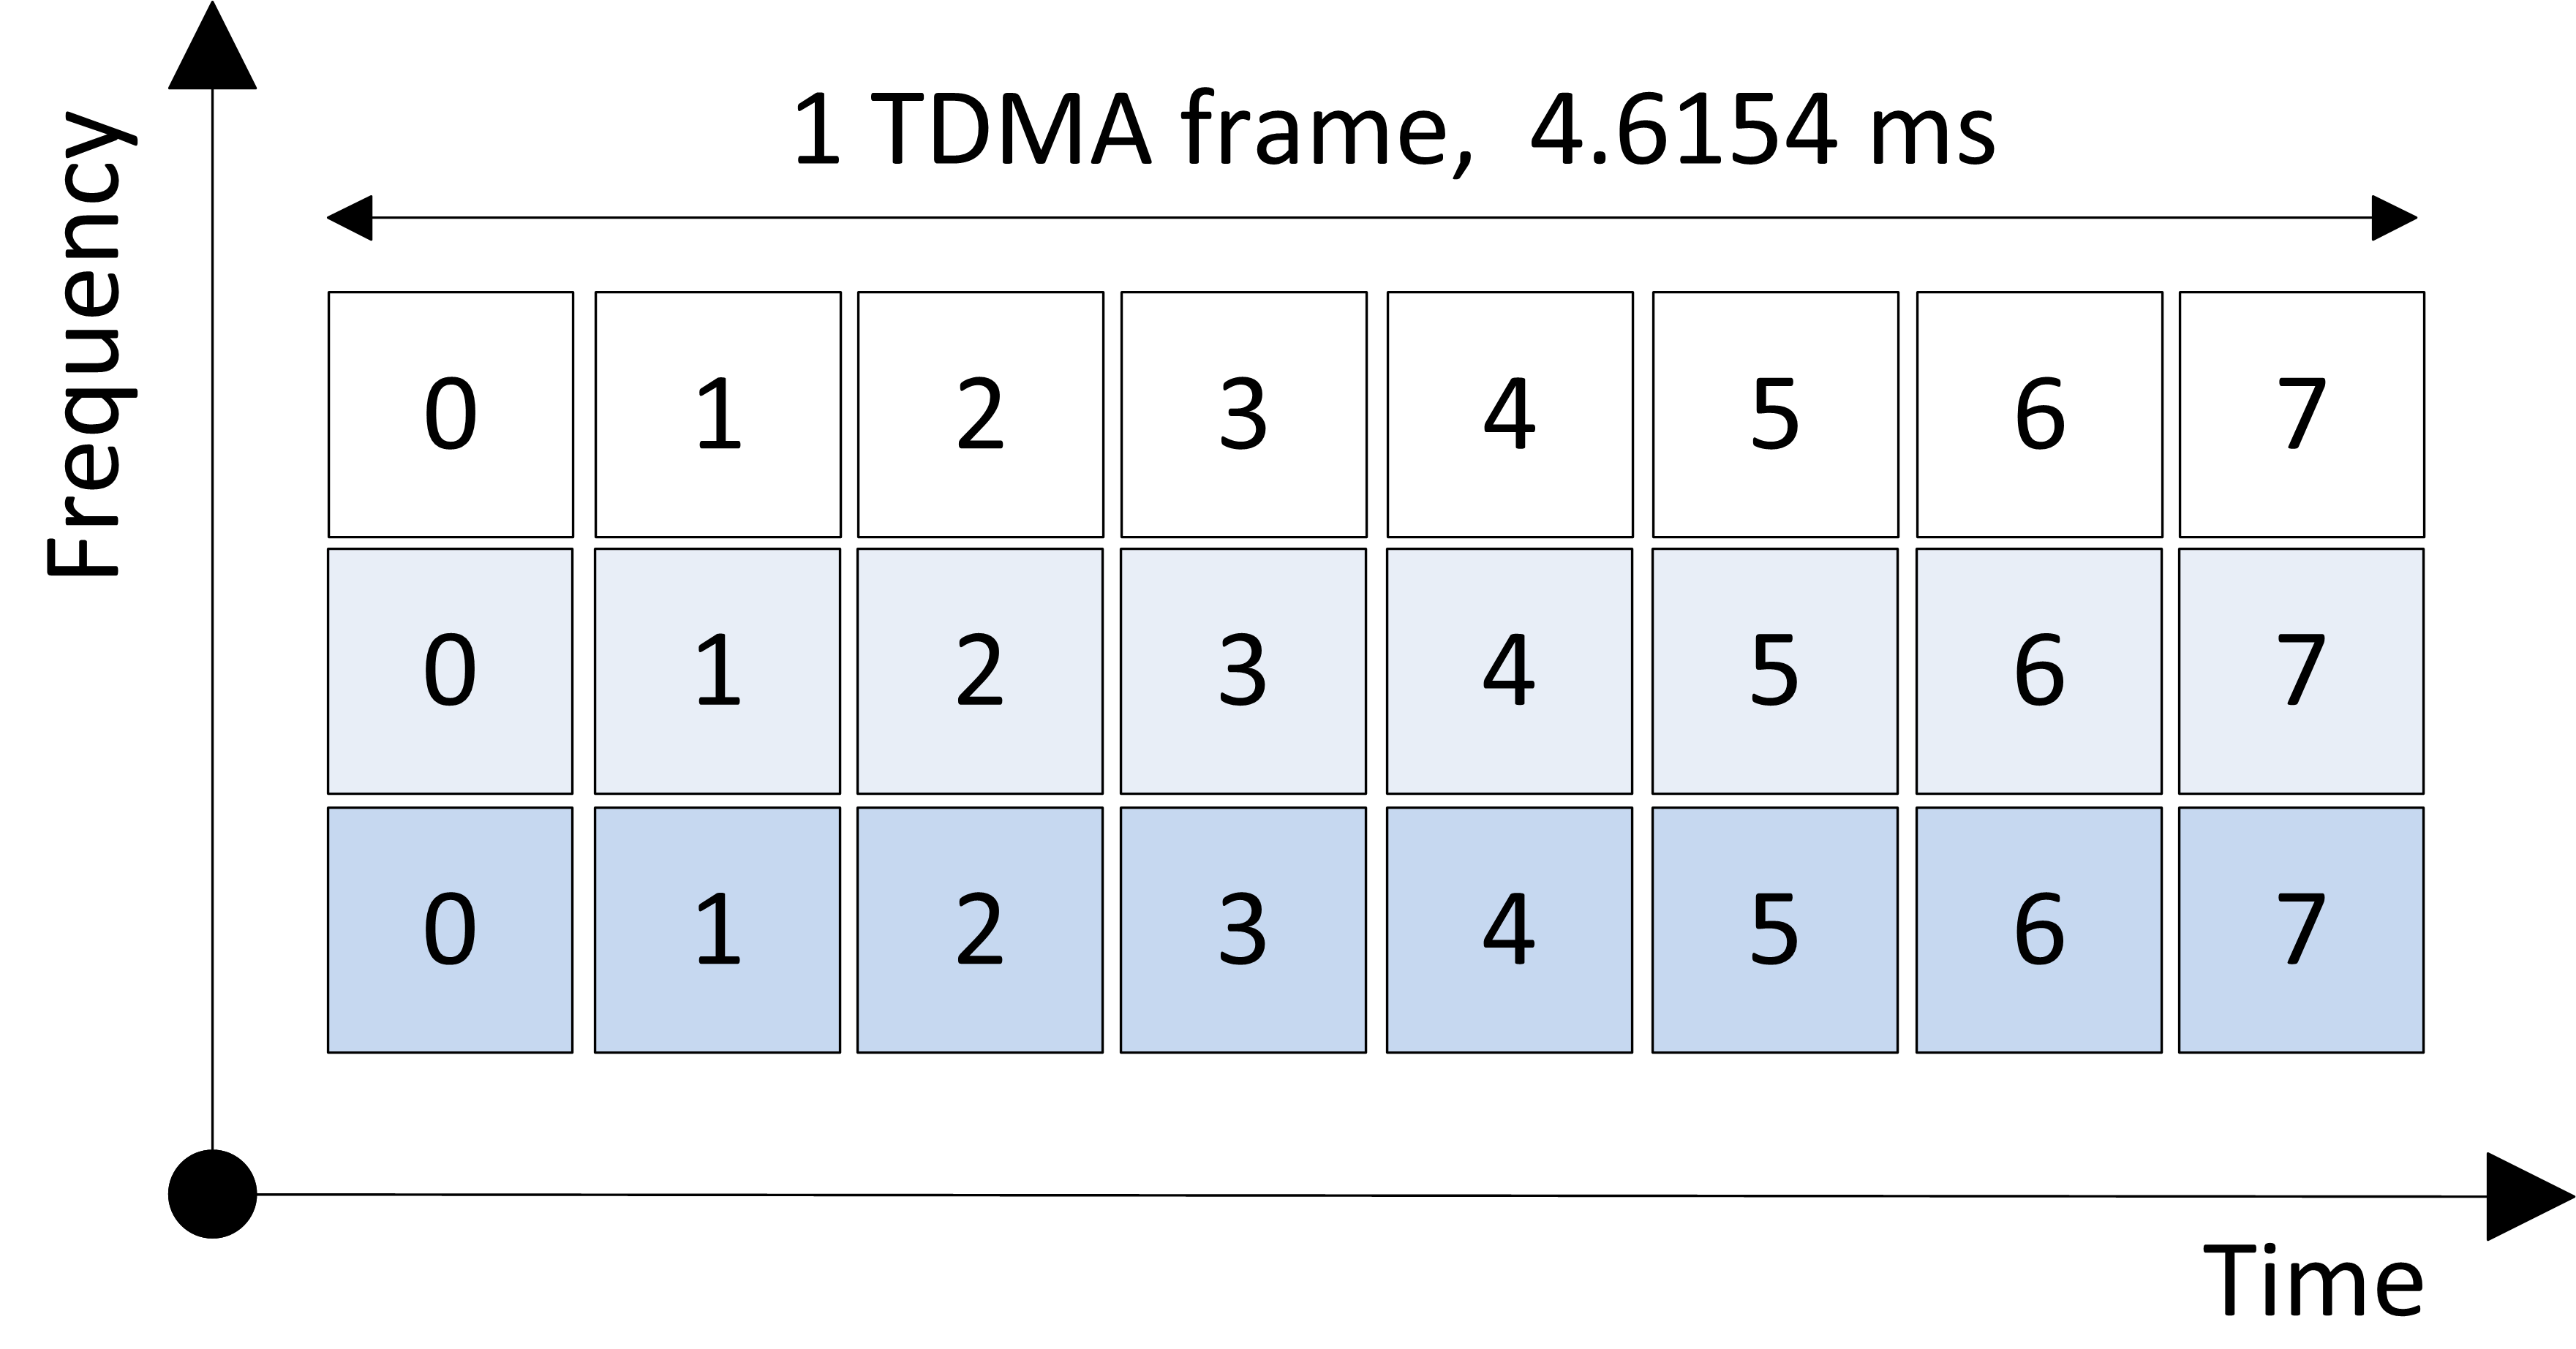
\includegraphics{../Images/TDMAFDMA}
	\caption{The combination of FDMA and TDMA.}
	\label{fig:fdma_tdma}
\end{figure}

\subsubsection{Frame Numbering}
Another important aspect is the frame hierarchy and the resulting frame numbering since it is used for ciphering as well as channel mapping and synchronisation.
The frame number is broadcasted frequently on the \gls{sch} to keep mobile subscribers in sync and inform subscribers that are about to connect or request a channel for communication.
Figure \ref{fig:frame_hierarchy} shows a complete diagram of the numbering scheme and frame hierarchy for reference.

The timeslots on the lowest level of the hierarchy have a length of $4.615\text{ ms} \div 8 = 577~\mu\text{s}$ and are also known as Bursts numbered from 0 to 7.
Every new \gls{tdma} frame the sequence number is increased by one.
Since this number cannot be increased endlessly is repeated every 3 h 28 m 53 s and 760 ms.
This is the largest chunk in the frame hierarchy and it is called Hyperframe.
Superframes and Multiframes are layers in between the Hyperframe and the \gls{tdma} frame.
As can be seen in the diagram the two variants of Multiframes, the 26-Multiframe containing 26 \gls{tdma} frames transports traffic channels as well as the respective control channels and the 51-Multiframe with its 51 \gls{tdma} frames with signalling data only.
Superframes wrap these different kinds of Multiframes into packages of the same size.
So either 51 26-Multiframes can be carried by a Superframe or 51 26-Multiframes yielding a duration of 6 s and 120 ms each.
Finally 2048 Superframes make up one Hyperframe.

\begin{figure}
	\centering
	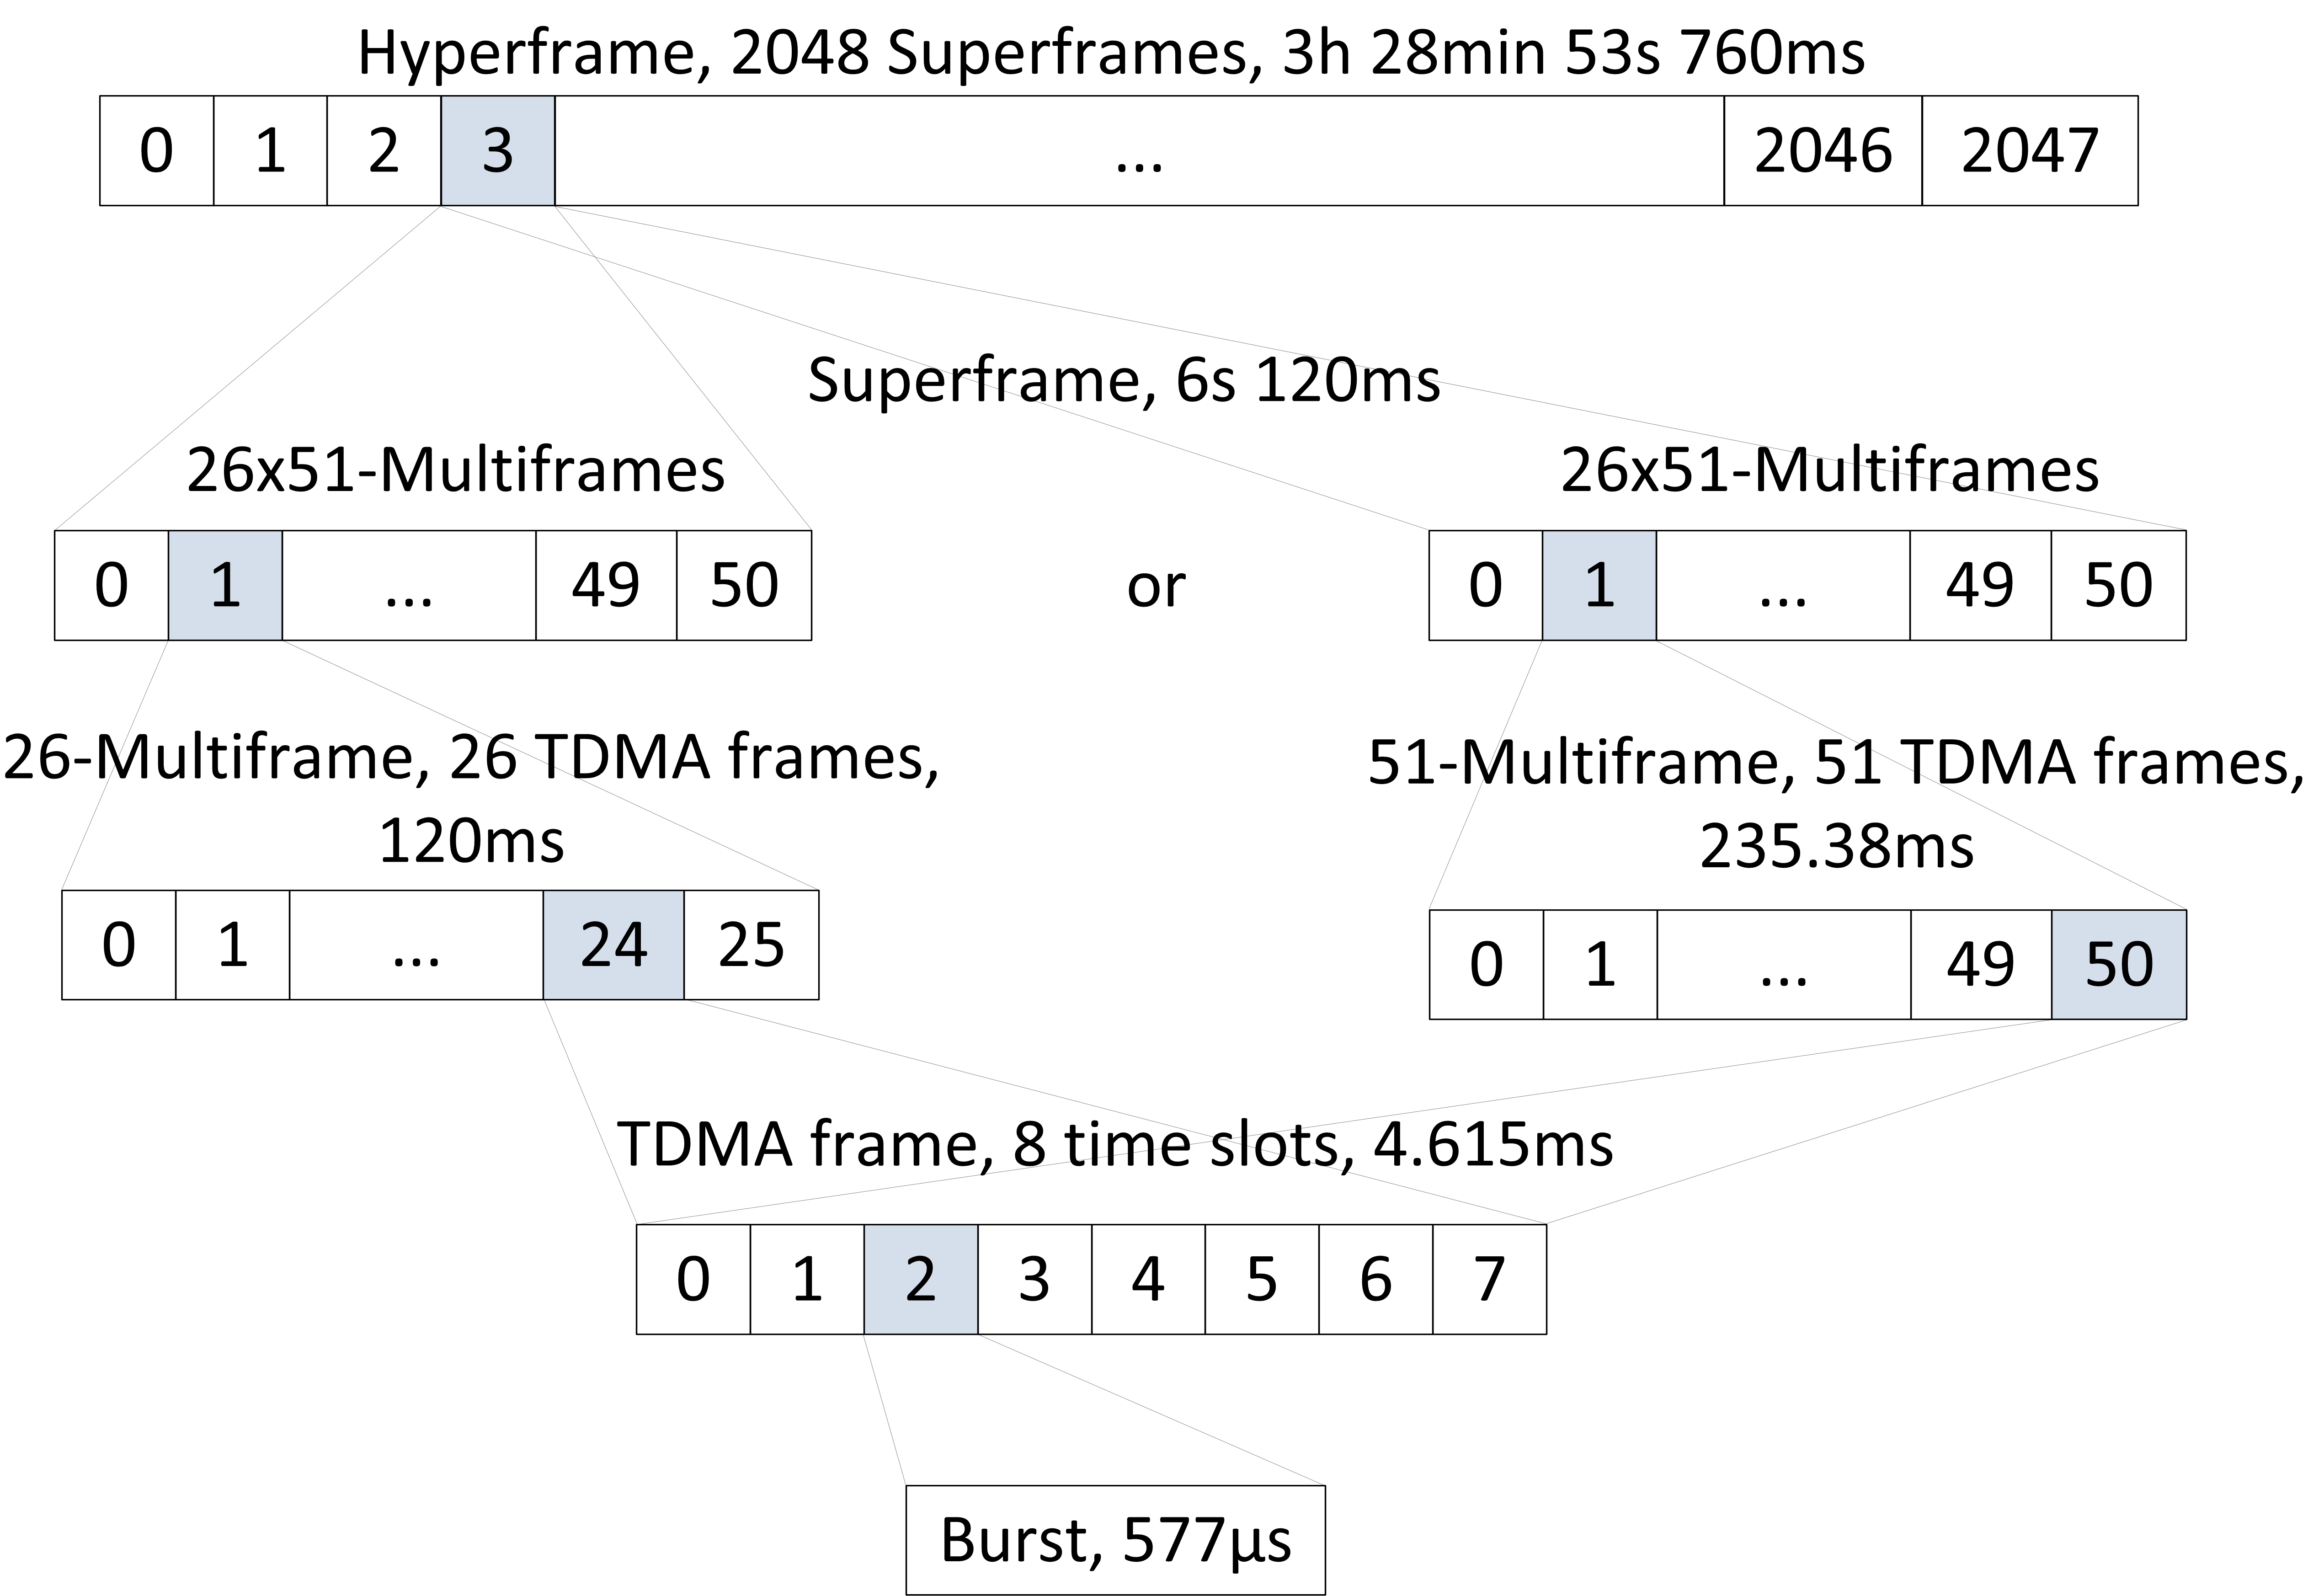
\includegraphics{../Images/Frames}
	\caption{Hierarchical Composition of the different frames.}
	\label{fig:frame_hierarchy}
\end{figure}

The frequency number thus is repeated every 3 hours this way which makes cracking the ciphering algorithm that has the sequence number as one of its inputs and thus intercepting a call considerably  more difficult.
When a \gls{ms} and \gls{bts} start to communicate the frame number has to be obtained by the \gls{ms} through the \gls{sch} before it can ask for a channel.
This is important since the frame number is a vital information indicating the chronological order of control channels.
If the \gls{ms} asks for a channel assignment in frame $n$ and a channel is assigned to the \gls{ms}, the assigned channels refers back to the frame $n$ and thus the \gls{ms} can find its channel amongst the others.

The last task mentioned above was synchronisation.
Since the mobile station and the transceiver station cannot send at exactly the same time, uplink and downlink of a channel are shifted by three timeslots.
The time in between uplink and downlink however cannot be fixed for all situations like that.
During a call a participant may move around and since radio waves travel at the speed of light slight variations in timing need to be dealt with.
If not data from two participants might overlap and be rendered unusable.
To avoid this problem each Burst has a Guard Time at the beginning and at the end, where no data is transmitted.
The complete structure of such a Normal Burst is outlined in Figure \ref{fig:burst_types}.
However this does not suffice if a subscriber moves away or to a \gls{bts} at considerable speed.
Therefore a mechanism called Timing Advance is used.
Basically the farther a subscriber is away from a base station the earlier a burst has to be sent, to compensate for the distance.
The value for the Timing Advance is determined by the \gls{bsc} after receiving a channel request message from the mobile station and afterwards constantly updated by the respective \gls{bts}.
The channel request message itself has only little data and large Guard Times since Timing Advance can only be used after this first measurement.

\begin{figure}
	\centering
	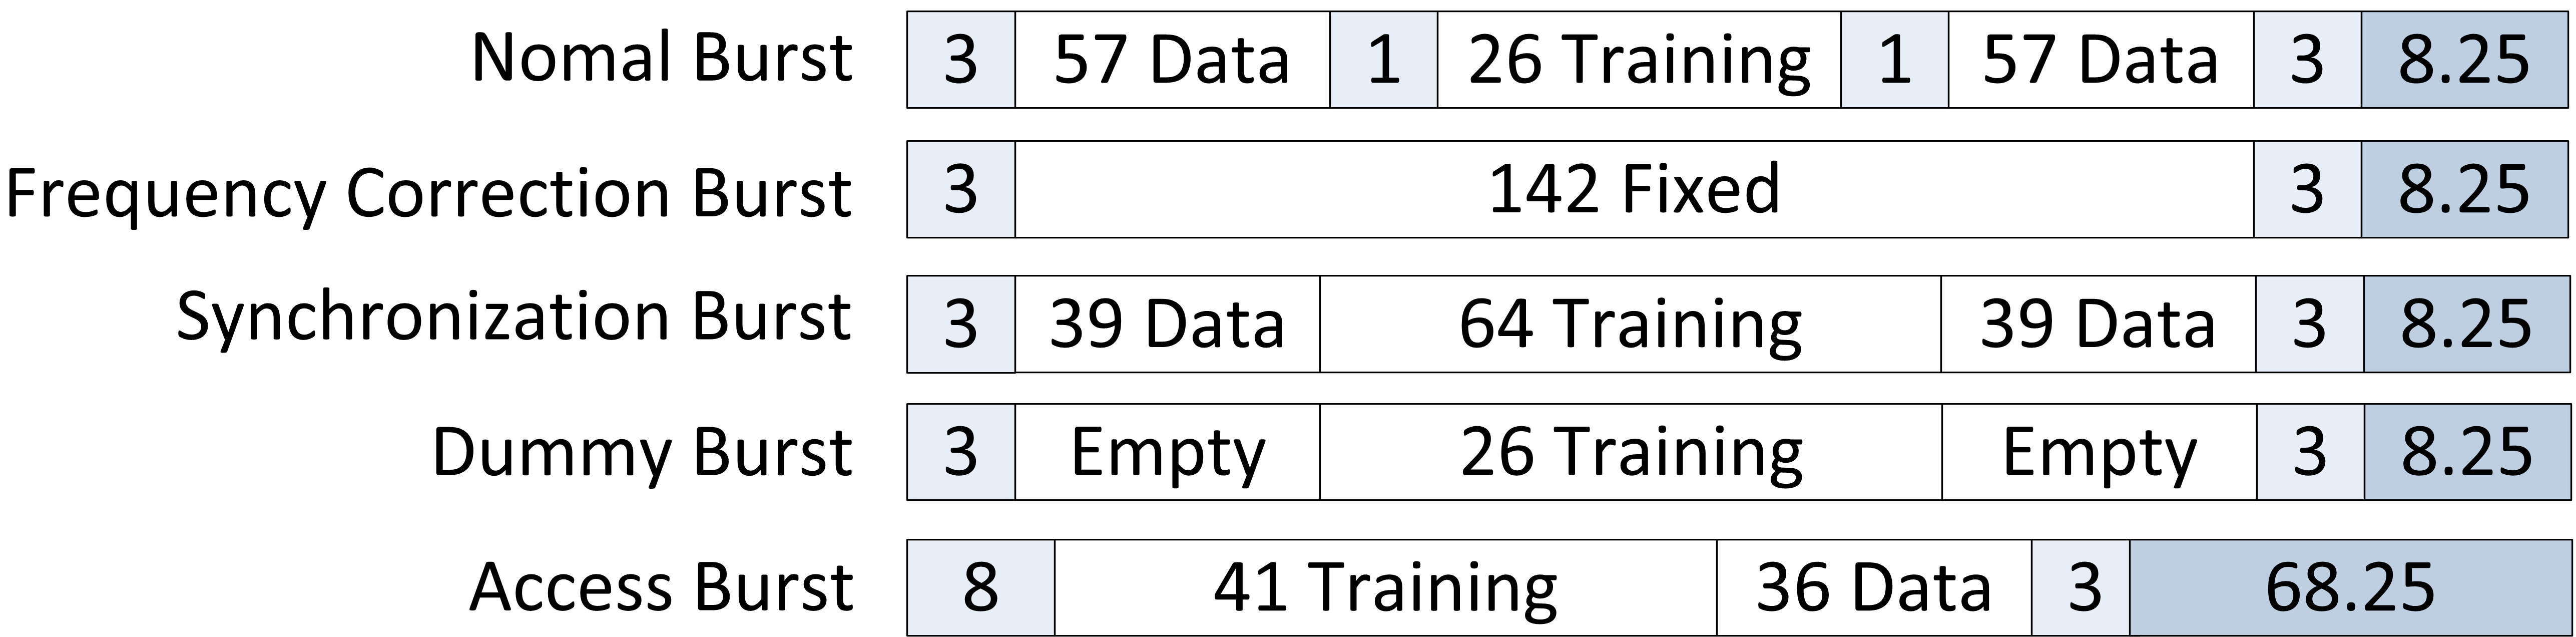
\includegraphics{../Images/Bursts}
	\caption{Structural Comparison of different Burst types. After \cite{GSM2009}.}
	\label{fig:burst_types}
\end{figure}

\subsubsection{Burst Types}
As suggested by the paragraph above there are different kinds of Bursts which are shown in \ref{fig:burst_types} \cite{GSM2009}.
All Bursts contain the before mentioned Guard Times which separate them from the next Burst.
In addition to data bits and known fixed bit sequences every frame has has tail bits, which mark the beginning and the end of a frame.
The training sequence is a fixed bit sequence that appears in conjunction with data bit sequences.
During a radio transmission procedure the signal can be distorted by shadowing, reflection, or other factors which would result in a loss of data.
But since the training sequence is known it is possible to reconstruct the original signal by comparing the incoming training sequence with the expected one and thus conserving the data bits.
\begin{itemize}
	\item Normal Burst: The basic information transmitting Burst.
	All information on traffic and control channels is transmitted by this Burst except for the \gls{rach}.
	Furthermore this Burst contains \glspl{sf}.
	If these are set the Burst contains important signalling data that has to travel fast over the \gls{facch} however no normal data can be transmitted in this case.
	\item Frequency Correction Burst: This Burst is sent frequently and is used by \glspl{ms} to fine tune to the frequency of the \gls{bts}.
	It may also be used by the \gls{ms} to do time synchronisation for \gls{tdma} frames.
	The periodic broadcasting of this frame is also called \gls{fcch} and shares a frequency with the \gls{bcch} as will be shown in the next section.
	\item Synchronisation Burst: This Burst contains time synchronisation information from the \gls{bts} to the \gls{ms} as well as the running \gls{tdma} frame number.
	Periodic broadcastings of this Burst form the \gls{sch}.
	\item Dummy Burst: When no other Bursts are sent on the frequency carrying the \gls{bcch} this one is transmitted to fill the gap.
	This way the \gls{ms} can keep up doing measurements even if no data needs to be transmitted.
	\item Access Burst: The Burst that is used to transmit data on the \gls{rach}.
	Since everyone can sent on the \gls{rach} without being given a timeslot via Slotted Aloha procedure the guard times of this Burst are high as to reduce the probability of data collisions.
\end{itemize}
The information in this section described the physical properties of the Air Interface also called Layer 1 when referring to the standard ISO/OSI model.
A short description of the other layers will be presented in Section \ref{sec:layers}.

\subsection{Logical Channels}
\label{sec:channels}
A logical channel is a virtual construct on top of the physical construct of frames to group similar information together.
Since not all information has to be sent all the time these different information channels, \eg broadcast information about the respective base station, can be multiplexed and sent together.
\begin{figure}
	\centering
	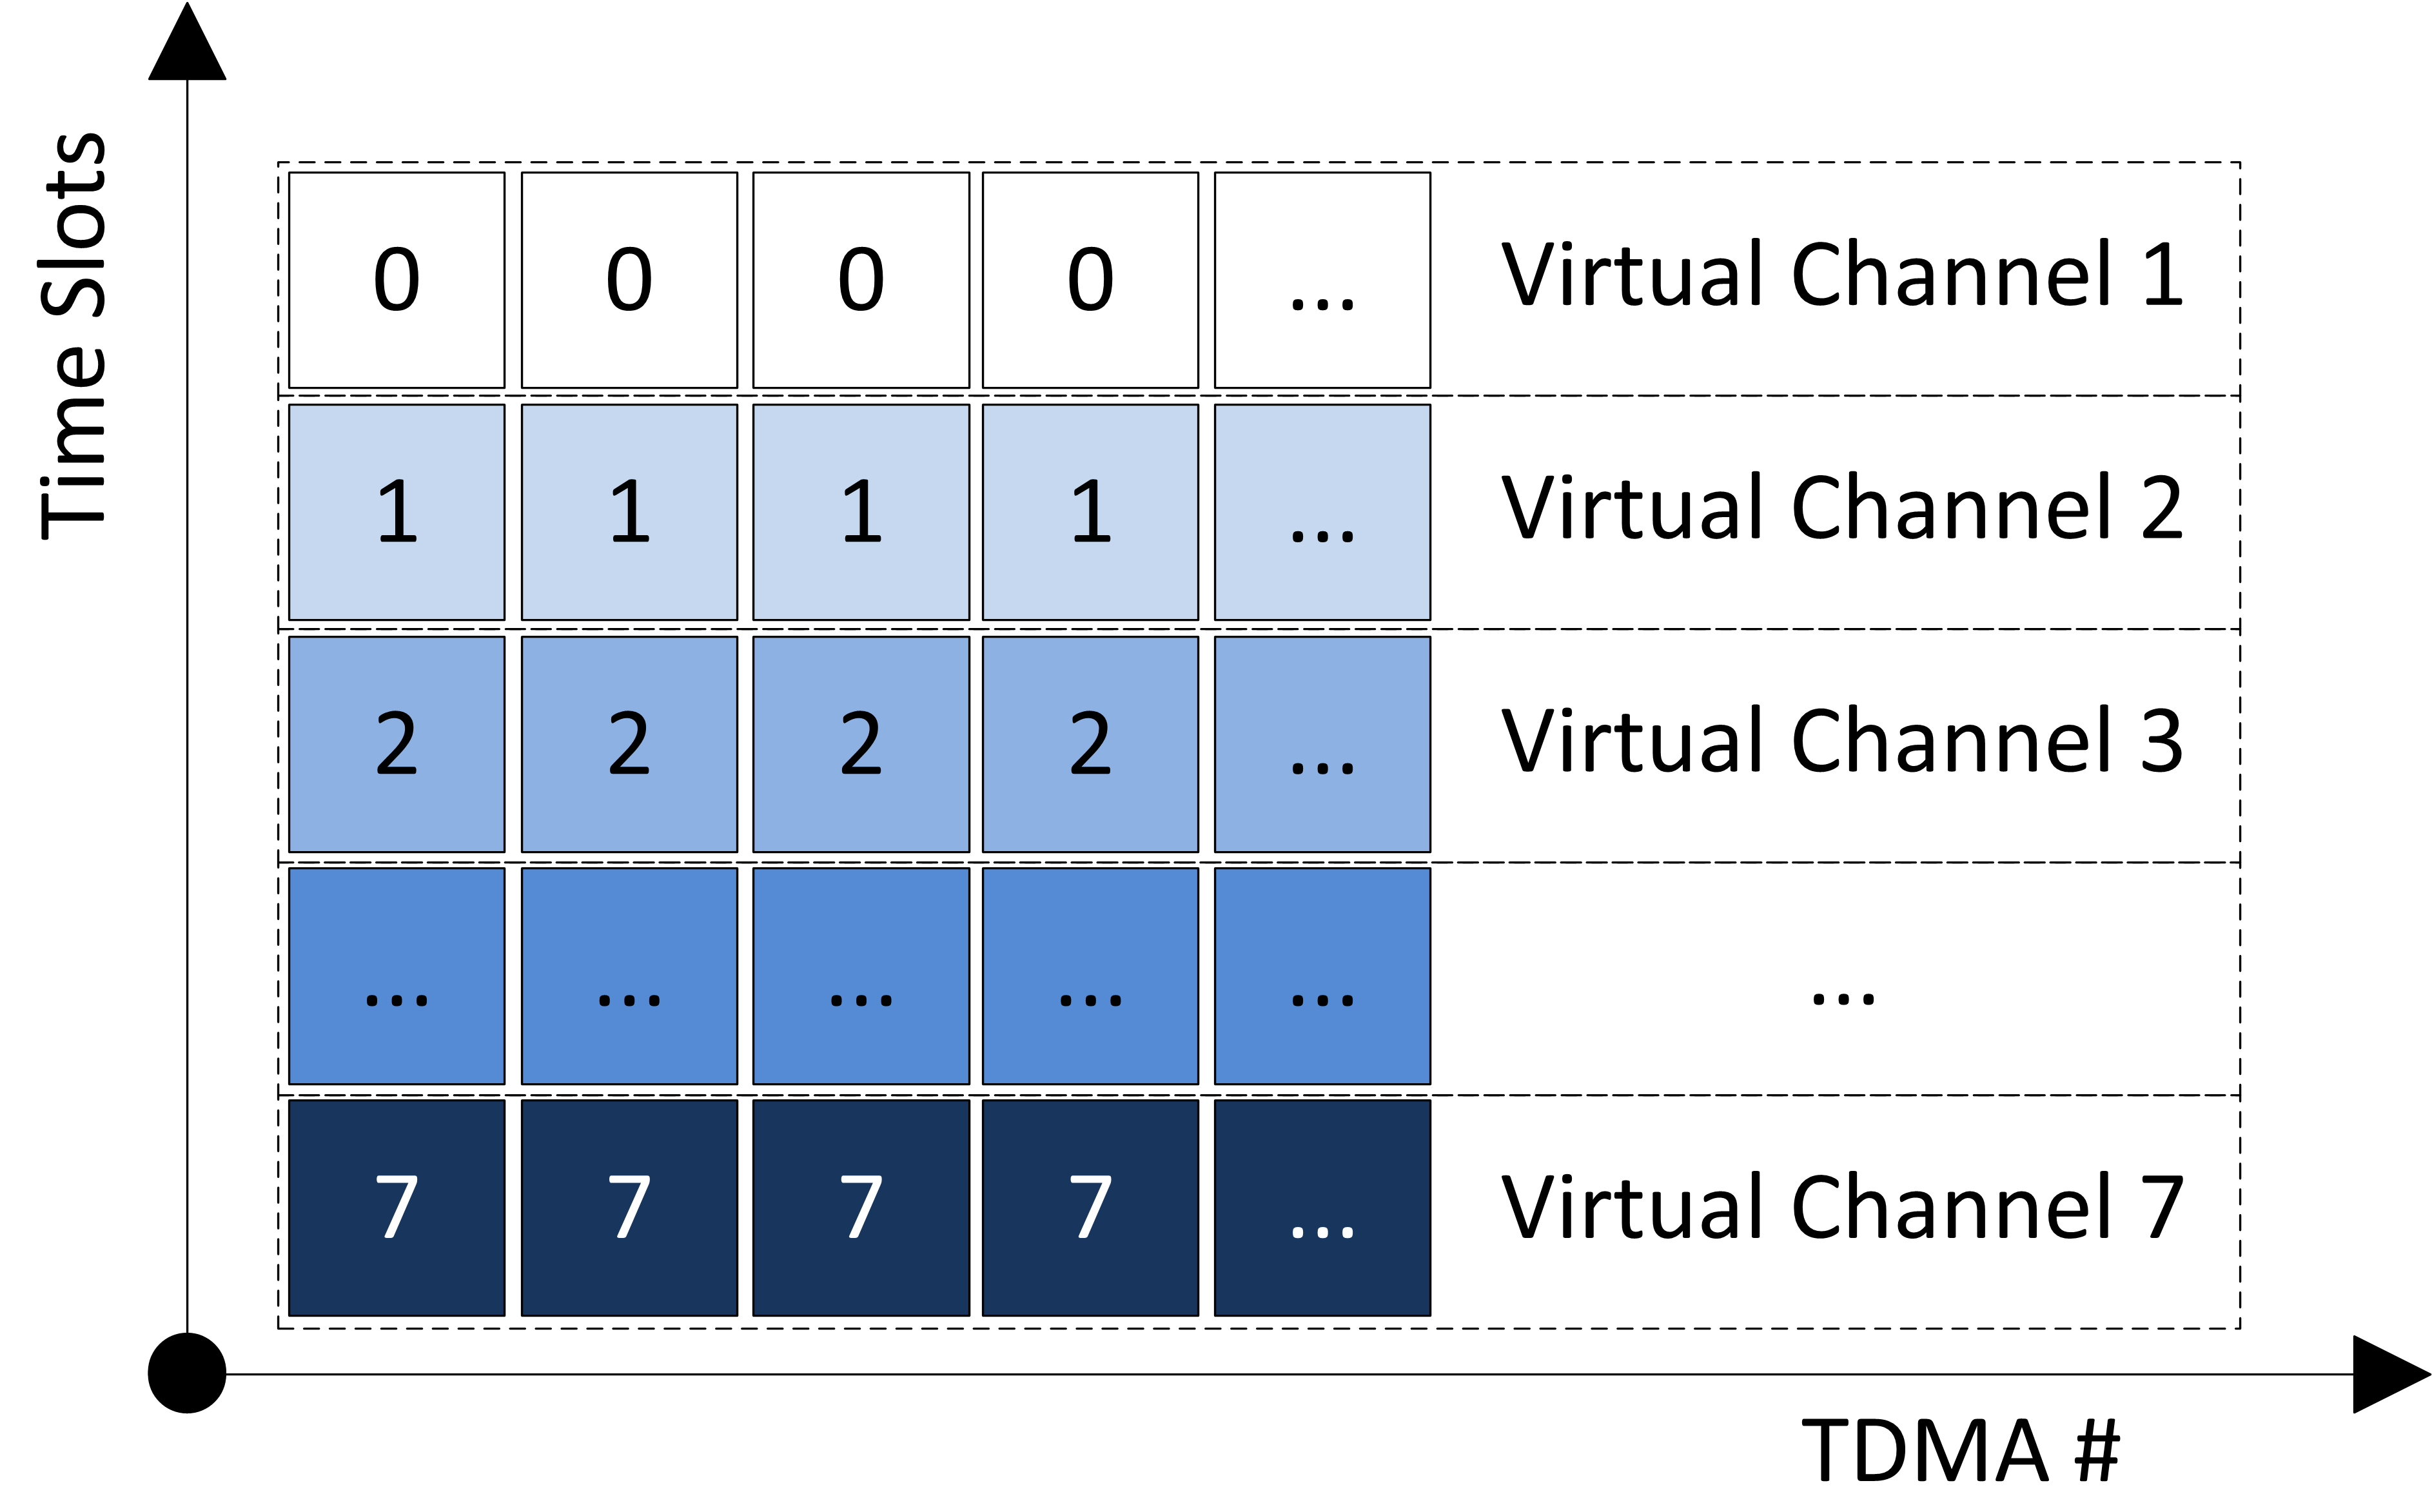
\includegraphics{../Images/Channels}
	\caption{Mapping of virtual channels on time slots.}
	\label{fig:channels}
\end{figure}

Mapping of these channels on the physical interface works in two dimensions.
The first dimension is frequency and the second is the time slot.
Figure \ref{fig:channels} shows this mapping of channels onto time slots over the course of multiple \gls{tdma} frames for one fixed frequency.
This way each timeslot over the course of multiple frames can be regarded as a virtual channel.
These resulting virtual channels can now be used by a multitude of logical channels to transmit information.

There are two main categories of logical channels distinguished by their usage \cite{kommsys2006}, dedicated channels and common channels.
Dedicated channels transport data meant for a single subscriber whereas common channels contain information interesting to all subscribers.

\subsubsection{Dedicated Channels}
As mentioned above, these channels wrap the communication of a single user with the network.
These are point to point channels.
\begin{itemize}
	\item \gls{tch}: A data channels that is used to transmit voice data or data service packages.
	\item \gls{facch}: A channel for transmission of urgent signalling data, \eg Handover signalling.
	This data doesn't have to be send often it shares a timeslot with the \gls{tch} and uses the stealing flags to insert its own data.
	\item \gls{sacch}: The uplink of this channel is used by the \gls{ms} to transmit quality measurements of the cell and neighbouring cells to the base station, so the network can do handover decisions accordingly.
	The downlink is used for Timing Advance data and power management data for the \gls{ms}.
	\item \gls{sdcch}: On this channel signalling information is sent to a subscriber as long as no \gls{tch} has been assigned during the initialisation of a call.
	Text messages and Location Updates are also transmitted on this channel.
\end{itemize}

\subsubsection{Common Channels}
The common channels contain data interesting to all subscribers, thus having a broadcast nature.
These are point to multi-point channels.
\begin{itemize}
	\item \gls{sch}: When the \gls{ms} is looking for a cell to connect, this synchronisation channel is used.
	\item \gls{fcch}: Used by \glspl{ms} to fine tune to the frequency of a certain base station and helps to find the start of a 51-Multiframe.
	\item \gls{bcch}: This channel is used to transmit information about the network and the base station itself through different system information messages.
	These contain the network name and cell identification as well as neighbourhood information on cells in the area and much more.
	This channel will be the main source of information for this project since it allows harvesting information without actively participating in the network and will thus be discussed in further detail in Chapter \ref{sec:info_gathering}.
	\item \gls{pch}: If a subscriber is not assigned a dedicated channel yet, \ie he/she is not active, they are notified on this channel if there is an incoming call or text.
	The subscribers are identified by their \gls{tmsi} which has been previously assigned upon entering the network so the \gls{imsi} does not have to be broadcasted.
	\item \gls{rach}: A subscriber that has been notified over the \gls{pch} can contact the network and request a \gls{sdcch}.
	Since this is a channel used by all connected and idle \glspl{ms}, access has to be regulated.
	As the name implies access is random thus it can happen that two or more \gls{ms} try to send at the same time.
	Slotted Aloha is used to handle access meaning there are fixed timeslots on which \glspl{ms} can send data.
	If collisions occur the data is discarded and each \gls{ms} has to wait a random time interval before sending again.
	\item \gls{agch}: This is the channel used to respond to a \gls{ms} if a request has been made on the \gls{rach}.
	The acknowledgement message also contains information on which \gls{sdcch} to use.
\end{itemize}
\subsubsection{Combinations}
These channels cannot arbitrarily be mapped onto Multiframes.
There is a complex multiplexing scheme defined in GSM 05.02 \cite{gsm0502} that explains which channel combinations can occur inside a Multiframe.
Since we are mainly interested in the downlink to harvest information from the \gls{bcch} Table \ref{tab:channel_configurations} shows the possible combinations of logical channels inside a  Multiframe on the downlink frequency.
\begin{table}
	\centering
	\begin{tabular}{lccccccccc}
	\toprule
						&M1&M2&M3&M4&M5&M6&M7&M8&M9\\
	\midrule
	TCH/F				&\cellcolor[gray]{0.7}&&&&&&&\cellcolor[gray]{0.7}&\cellcolor[gray]{0.7}\\
	TCH/H				&&\cellcolor[gray]{0.7}&\cellcolor[gray]{0.7}&&&&&&\\
	TCH/H				&&&\cellcolor[gray]{0.7}&&&&&&\\
	BCCH				&&&&\cellcolor[gray]{0.7}&\cellcolor[gray]{0.7}&\cellcolor[gray]{0.7}&&&\\
	FCCH				&&&&\cellcolor[gray]{0.7}&\cellcolor[gray]{0.7}&&&&\\
	SCH					&&&&\cellcolor[gray]{0.7}&\cellcolor[gray]{0.7}&&&&\\
	CCCH				&&&&\cellcolor[gray]{0.7}&\cellcolor[gray]{0.7}&\cellcolor[gray]{0.7}&&&\\
	SDCCH				&&&&&\cellcolor[gray]{0.7}&&\cellcolor[gray]{0.7}&&\\
	SACCH				&\cellcolor[gray]{0.7}&\cellcolor[gray]{0.7}&\cellcolor[gray]{0.7}&&\cellcolor[gray]{0.7}&&\cellcolor[gray]{0.7}&\cellcolor[gray]{0.7}&\cellcolor[gray]{0.7}\\
	FACCH				&\cellcolor[gray]{0.7}&\cellcolor[gray]{0.7}&\cellcolor[gray]{0.7}&&&&&\cellcolor[gray]{0.7}&\\
	\midrule
	Multiframe Type		&26&26&26&51&51&51&51&26&26\\
	\bottomrule
	\end{tabular}
	\caption{Possible combinations of logical channels for the base station. From \cite{GSM2009}.}
	\label{tab:channel_configurations}
\end{table}
The mapping of these specific Multiframe-configurations onto timeslots is not arbitrary either.
Normally TS-0 and TS-1, the first two time slots, are used handle channels with signalling information.
The \gls{bcch} for example uses TS-0 of the carrier frequency.

Figure \ref{fig:channel_example} shows an example \cite{kommsys2006} for the downlink of a base station where these channel configurations can be seen.
As mentioned before, TS-0 and TS-1 are used for signalling purpose where the Multiframe-configurations M5 and M7 can be found respectively.
The slots for the \gls{bcch} can be seen here.
The table shows, that these configurations do not contain any traffic channels.
As for traffic channels, TS-2 through to TS-7 are used with the configuration M1 or M3.
It cannot be seen from the data whether full rate or half rate channels are used for transporting voice data but since half rate channels are not used very often \cite{protocols1999}, it is more likely that it resembles M1.
\begin{figure}
	\centering
	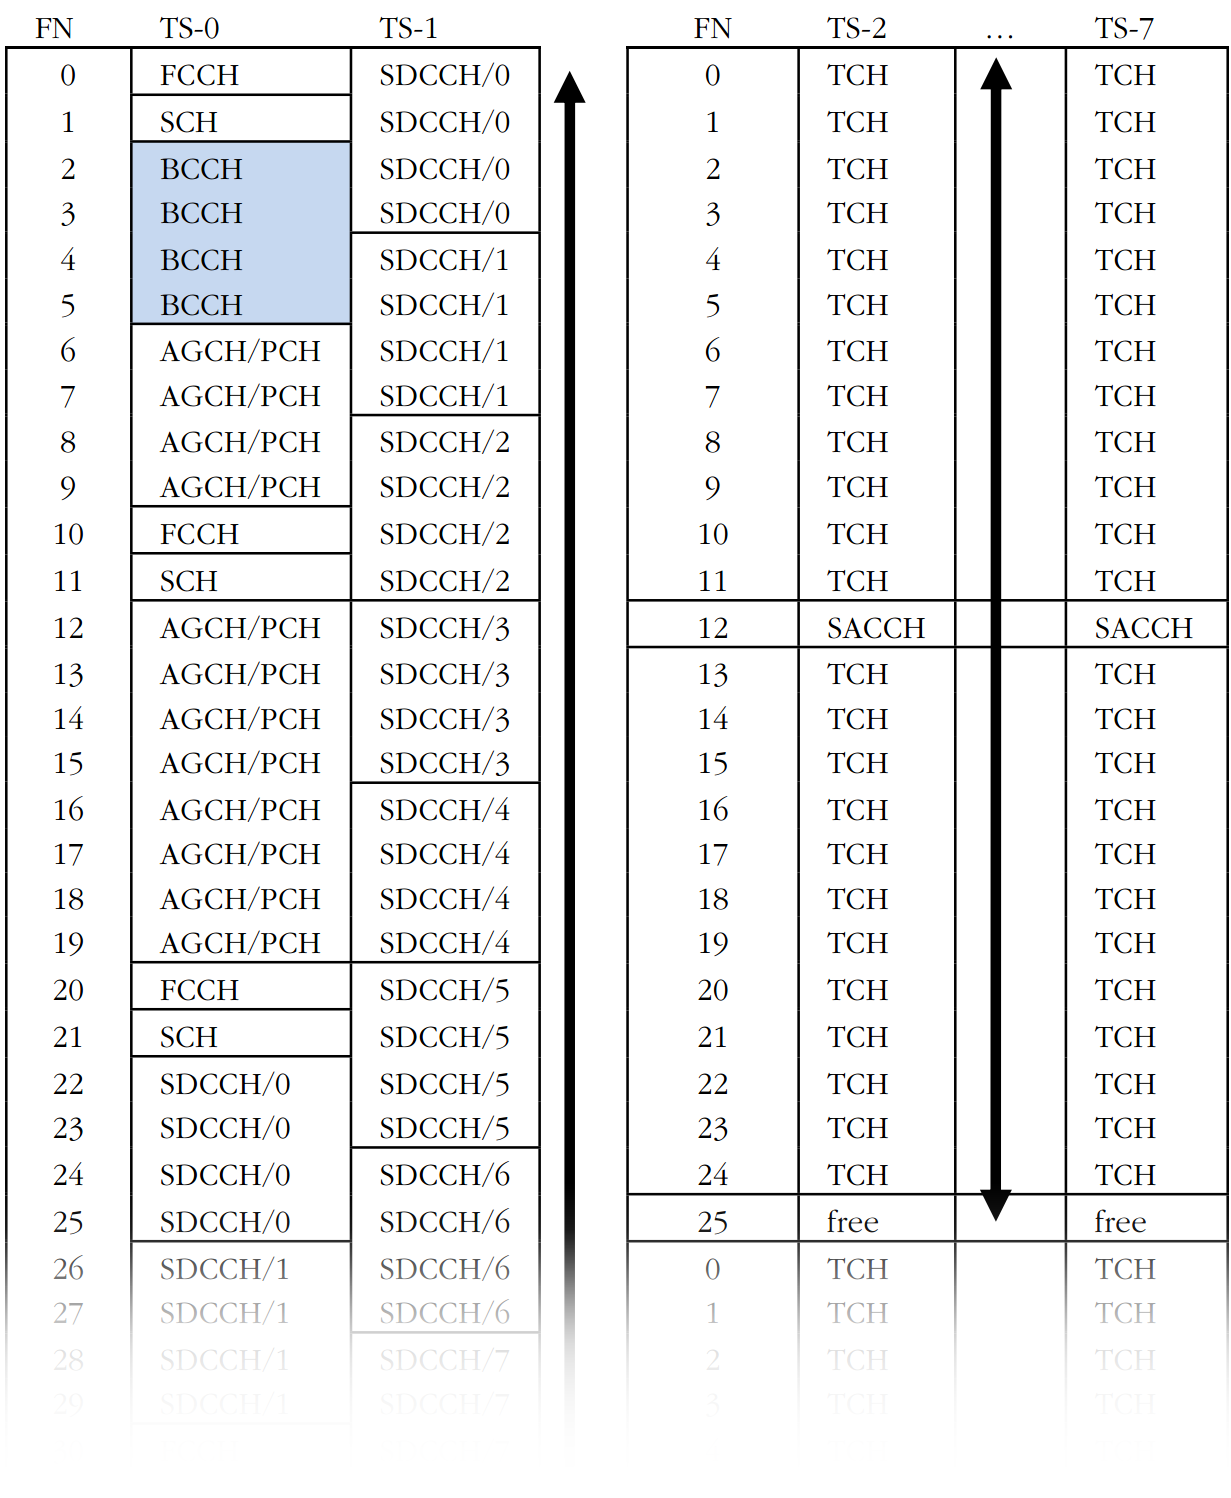
\includegraphics[width=.9\textwidth]{../Images/channel_example}
	\caption{Snippet of a Multiframe-configurations for a base station from \cite{kommsys2006}.}
	\label{fig:channel_example}
\end{figure}

\subsection{Layers}
\label{sec:layers}
Design-wise the layers of the $U_m$ interface resemble the layers of the ISO/OSI model reference model specified by the \gls{itu}.
This section will give a short overview over the first three layers with respect to the air interface \cite{protocols1999}.
It is important for further understanding to know what functionality can be found on which of the three lower layers, since the framework employed to gather information in this project will directly work on and with those layers.

\paragraph{Physical Layer (Layer 1):} This layer provides the facilities for the actual transmission of data.
In case of the $U_m$ interface this is the actual radio equipment.
This layer does not know data types like user or signalling data.
The data that it receives from Layer 2 are either single bits or an array of bits.
On the algorithmic side of the $U_m$ interface the \gls{gmsk} modulation that is used to encode the data of a Burst into radio signals is part of Layer 1.

\paragraph{Data Link (Layer 2):} On Layer 2 packaging is done.
The notion of data frames is introduced to have chunks of information on which error checking and potential retransmission of corrupted data can be performed.
The Layer 2 protocol \gls{hdlc} is used as a basis for \gls{ss7} as well as for \gls{lapd}.
\gls{hdlc} and its derivatives use start/stop markers and checksums to form data frames.
The Layer 2 format changes through the course of the network while the data packages of layer 3 may stay the same.
When a transmission from a \gls{ms} to the \gls{bts} is done \gls{lapdm} is used which is essentially the same as the Layer 2 \gls{isdn} protocol with a few simplifications.
From the \gls{bts} to the \gls{bsc} \gls{lapdm} converts to \gls{lapd} and afterwards is exchanged to \gls{mtp2}.
For the air interface \gls{lapdm} along with channel coding and Burst formatting form Layer 2.
More information about these Layer 2 protocols can be found in the respective Technical Specifications of the \gls{3gpp} \cite{GSM0405,GSM0406}.

\paragraph{Network (Layer 3):} Layer 3 headers have to provide all the information necessary for the packet to be routed towards its recipient.
As with Layer 2 information it may be the case that this header needs to be partially rewritten during the transmission of a package.
Between the \gls{ms}, \gls{bts}, \gls{bsc} and \gls{msc} the \gls{rr} protocol and the information needed to route a call into the \gls{ss7} subsystem are part of Layer 3.
This protocol handles configuration and allocation of radio channels as well as managing the dedicated channels to the subscribers.
Therefore in a strict sense \gls{mm} and \gls{cc} information does not belong to Layer 3 functionality but is only transported via \gls{rr} between \gls{ms} and the \gls{nss} \cite{protocols1999}.

\section{IMSI-Catcher}
\label{sec:catcher}
An \gls{imsi}-Catcher is a technical device that is used to capture the \gls{imsi} and \gls{imei} numbers of mobile subscribers.
The knowledge of the \gls{imsi} and \gls{imei} numbers can be exploited to either tap into the participant's calls or pinpoint the location of the subscriber \cite{fox}.
Another less known functionality is that if catchers do not relay intercepted calls they can be used to suppress mobile communication in a certain area \eg during a police operation \cite{imsi_wiki}.

This topic came up in conjunction with crime fighting and prevention with the advent of mobile telephones.
A mobile phone cannot be tapped in the same way as a landline phone since the subscriber can change places and also phones thus there is no designated line associated with him/her.
This has proven to be a challenge to the authorities.

In 1996 Rohde \& Schwarz a company based in Munich, Germany has developed a device called ''GA 090'' which was the first \gls{imsi}-catcher.
Its was capable of yielding a list with all the \gls{imsi} numbers in the perimeter as well as pinpointing the location of a subscriber given the \gls{imsi}.
Short thereafter the ''GA 900'' was presented which had the additional capability of tapping into calls that originated from a particular \gls{imsi}.
These commercial versions of catchers produced by Rohde \& Schwarz were priced between 200 000 \euro{} and 300 000 \euro{} in 2001 \cite{fox}.
Although these catchers are meant to be bought by authorities, it is also possible to buy them as a private customer or to order them from abroad.
Regulations prohibit the use of \gls{imsi}-catchers for individuals since the frequency bands the \gls{gsm} network uses are reserved for providers.
However it cannot be guaranteed that such a catcher is not used illegally.
In addition to these commercial products different projects \cite{dennis, def_catcher} have shown that such devices can be built at a very low budget.
This only intensifies the risk that is imposed by the abusive usage of such a catcher.
Figure \ref{fig:catchers} shows a commercial model side by side with a self built catcher.
\begin{figure}
\centering
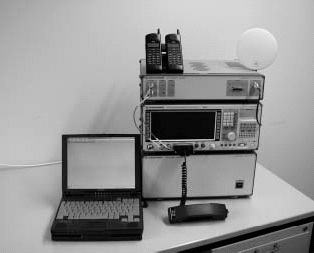
\includegraphics[width=0.45\textwidth]{../Images/imsi_catcher}\hspace{1cm}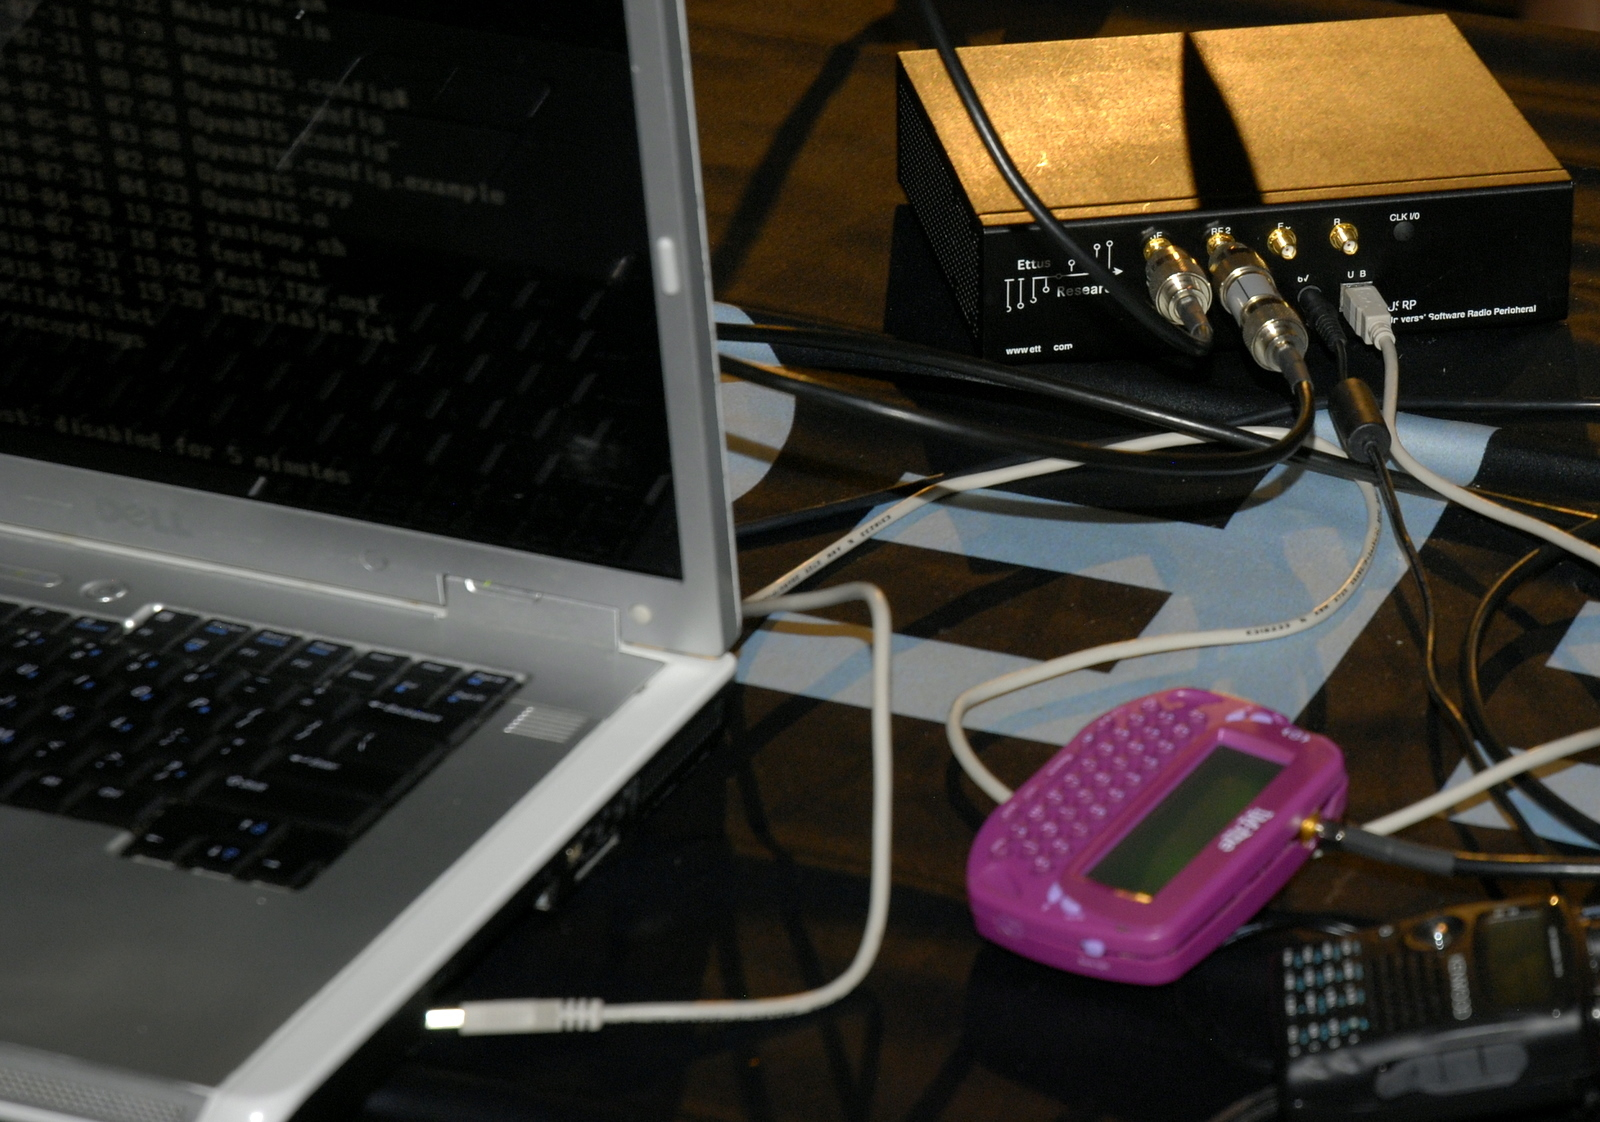
\includegraphics[width=.45\textwidth]{../Images/usrp}
\caption{A commercial catcher by Rhode \& Schwarz \cite{fox} and a self built catcher introduced at Defcon 2010 \cite{def_catcher}.}
\label{fig:catchers}
\end{figure}

Section \ref{sec:catcher_operation} will show how an \gls{imsi}-catcher works and how subscribers can be caught.
In addition the potency of these attacks will be evaluated and what risks these impose from a technical perspective.
The next section will explain under which circumstances a catcher can be used in Germany from a legal perspective and show that this handling poses the risk of privacy breach to citizens.

\subsection{Mode of Operation}
\label{sec:catcher_operation}
Basically an \gls{imsi}-Catcher masks itself as a base station and lures subscribers in its perimeter, to connect to it without their knowledge.
Ways of luring a subscriber into a catcher are explained in Section \ref{sec:attacks}.
The one shown in Figure \ref{fig:catcher_catch} is broadcasting a new \gls{lai} to the \gls{ms} at very high power, suggesting that the \gls{ms} entered a new area and has to re-authenticate \cite{mueller}.

\begin{figure}
	\centering
	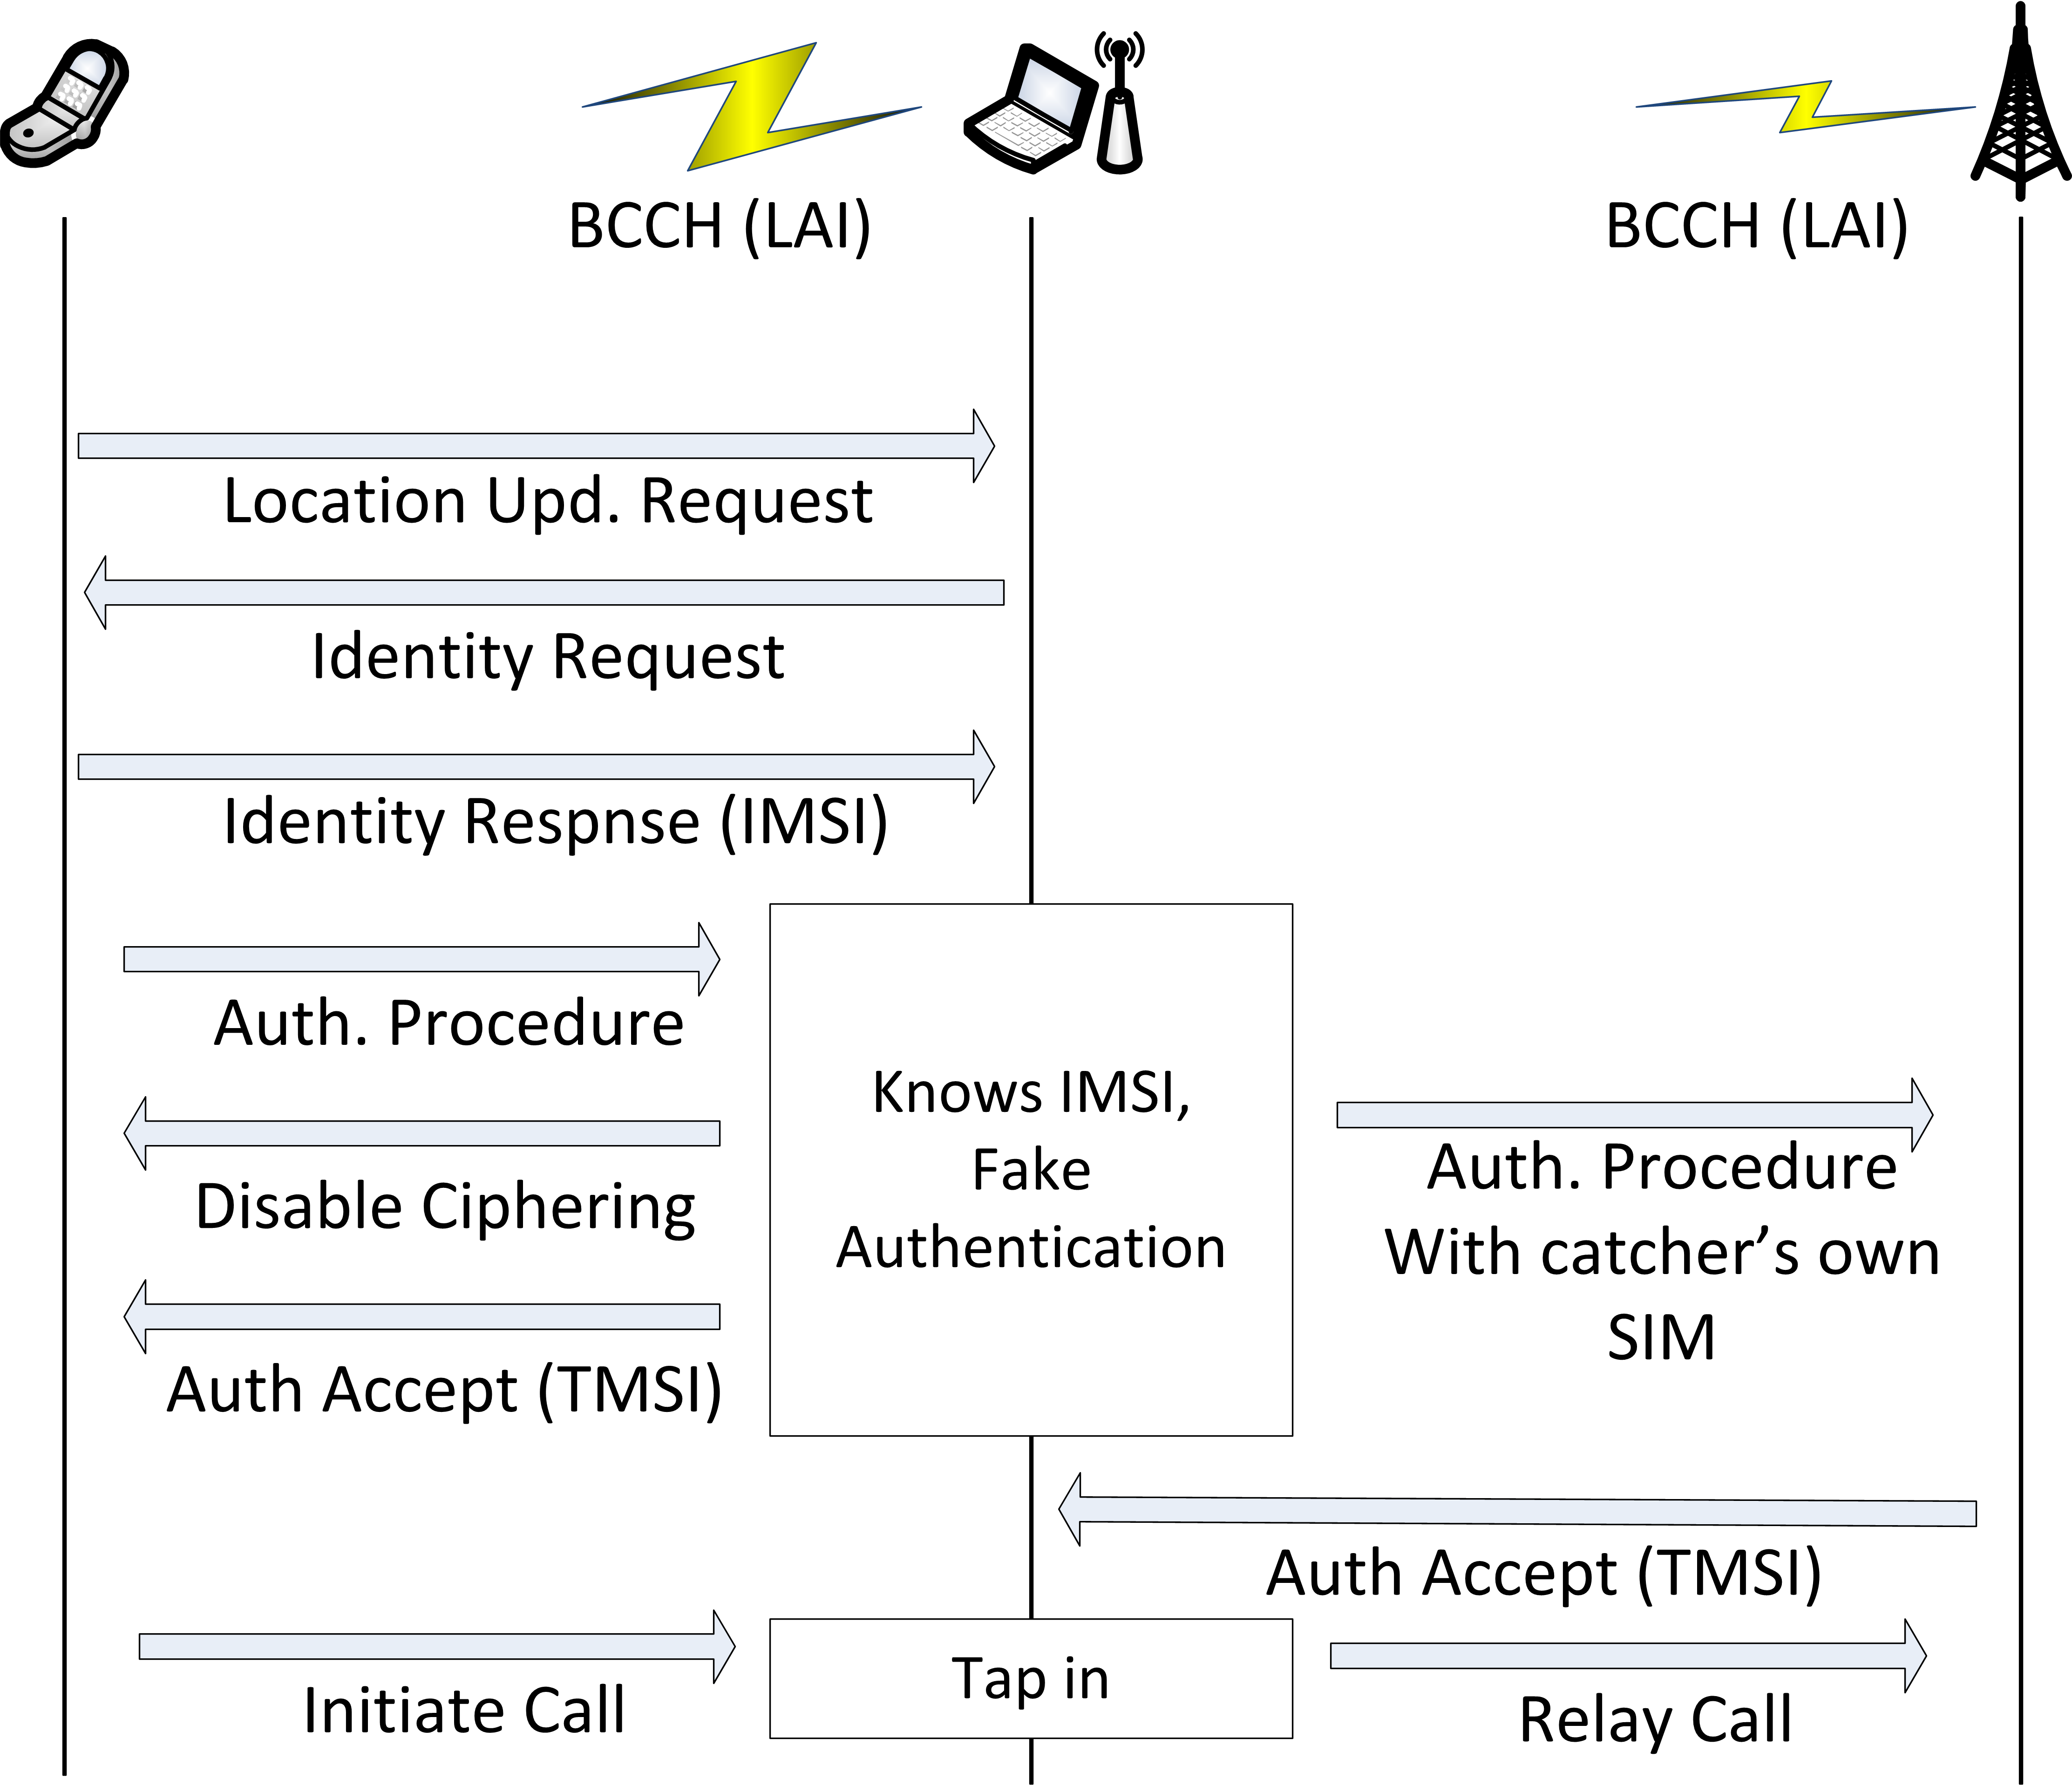
\includegraphics{../Images/catcher_attack}
	\caption{IMSI catching procedure. Adopted and simplified from \cite{mueller}.}
	\label{fig:catcher_catch}
\end{figure}

Once a subscriber connects to the device, a command is sent to the \gls{ms} which asks for the \gls{sim}'s \gls{imsi}.
This command is normally only used in case of an error \cite{fox} but can be abused this way.

This is only possible since authentication in a \gls{gsm} network is one-sided as discussed earlier in Section \ref{sec:authentication}.
The subscriber has no way of checking the authenticity of a base station but rather has to trust the broadcasted identifier which can be easily forged by a catcher.
At this stage, the subscriber can already be localized as being in a certain distance of the catcher.

Having the \gls{imsi} the authorities can now also query the provider for personal information about the subscriber, however criminals often use fake credentials when obtaining a \gls{sim} card.
Since it is only possible to catch all the \glspl{imsi} in an area, the person to be observed has to be followed and the catcher has to be used multiple times.
Each time it yields a set of numbers in the area. 
The \gls{imsi} that is part of all the sets is the \gls{imsi} of the person under observation.
More catchers can now be used to triangulate the position.
The next step is also possible because of a design decision made in the \gls{gsm} protocol.
Encryption itself or certain kinds of strong encryption are not allowed in all countries.
Therefore it is possible for the base station to request the encryption algorithm A5/0 which means that no encryption will be used for the calls at all.
Only a few mobile phones display that encryption has been disabled by the \gls{bts}.

At this point the setup for a man-in-the-middle attack \cite{mueller} on calls is completed.
The catcher itself is connected to the mobile network with its own \gls{sim}.
If the subscriber now initiates a call, the call can be routed by the catcher into the network and since encryption is turned of it can also be listened to or recorded.
The subscriber doesn't notice this privacy breach except in the rare cases where the phone displays that encryption has been turned off.
The \gls{imei} is also harvested in a similar fashion if the observed person tries to switch \gls{sim} cards on a regular basis \cite{fox}.

\subsubsection{Attacks}
\label{sec:attacks}
When operating a catcher the first and most important step is to actually trick the \gls{ms} into connecting to the catcher.
A lot of phones save the frequency the were tuned to last and upon connecting to the mobile network this is the first frequency they try.
Therefore a \gls{ms} has to be set to 'normal cell selection' mode which means it starts scanning for the best base station available.
Four possible ways of luring a \gls{ms} to the \gls{imsi}-catcher will now be explained.
Three were presented by Wehrle for the 'Open Source IMSI-catcher' project \cite{dennis} and one by Federrath \cite{mueller}.
The attacks differ on whether the \gls{ms} already is in normal cell selection mode or not, \ie it is connected to another \gls{bts}.

\paragraph{\gls{ms} is in normal cell selection mode:}
The \gls{imsi}-catcher has to emulate a cell configuration of the provider the target \gls{ms} is looking for broadcasting at any frequency.
If the \gls{ms} stumbles upon the frequency it will connect.
This is no method with 100\% accuracy however chances can be raised by broadcasting with higher power.
Some \gls{imsi}-catchers even broadcast at a higher power than it would be allowed for normal \gls{bts} \cite{imsi_wiki} to make certain to be the strongest base station available to the \gls{ms}.

\paragraph{\gls{ms} is already connected to a network:}
If this is the case then the connection to the current cell needs to be broken.
It can be achieved either by jamming the frequency band of the cell the \gls{ms} is connected to thus forcing the \gls{ms} into cell selection or by getting the \gls{ms} to switch the cell to the catcher's.
This can be done the following way.
In this method the fact is abused that the \gls{ms} knows its neighbourhood (since it has been broadcasted by the \gls{bts}) and does regular quality measurements.
The main idea is that the operator of the catcher chooses the frequency of a \gls{bts} that is in the neighbourhood of the \gls{bts} that the target \gls{ms} is connected to.
This way the operator can make sure the \gls{ms} know this frequency and hast quality measurements associated with it.
Furthermore should the chosen \gls{bts}, the one that will be replaced by the catcher, have a bad signal to noise ratio (which is why the \gls{ms} is currently not connected to it).
As soon as the catcher starts broadcasting on that frequency, quality measurements will radically improve and the \gls{ms} will initiate a change of cells to the catcher cell if the quality is above its current cell.
Another way is to broadcast a new \gls{lai} to the \gls{ms} suggesting it just arrived at a new location and therefore initiating a cell selection \cite{mueller}.
This works as long as the \gls{ms} has no active connections to the network, if it has, the jamming method can help to disconnect the \gls{ms} from the network.

\subsubsection{Risks and Irregularities}
An \gls{imsi}-catcher cannot target an individual subscriber, it always targets an area thus breaching the privacy of uninvolved subjects.
Apart from that, a catcher that does not relay calls takes away the possibility for all connected people in the area to initiate calls.
Even if the the catcher routes calls into the network, since it only has one \gls{sim} card, it can only route a single call.
This can be very dangerous because no emergency calls can be submitted in that area during the time of operation which can be as long as five to ten minutes \cite{fox}.

Another irregularity apart from using no encryption is that people caught in this area cannot be reached on their mobile phones since they are not registered on the main network.
As a consequence of the proxy functionality of the \gls{imsi}-catcher, when a call is routed into the network the recipient can only see the number the catcher is registered with or 'Number Withheld' however not the original number.

\subsection{Law Situation in Germany}
\label{sec:catcher_law}

First reports of an \gls{imsi}-catcher used by authorities in Germany dates back to 1997.
Until November 2001 35 cases of use were officially confirmed by the \gls{bmi} \cite{fox}.
It was used to fight of organised and serious crime like hostage-takings or drug traffic by the \gls{bka} and \gls{bgs}.
Attempts have been made by the government to move the catcher out of the legal grey zone and use the 'GA 900' with its capabilities of tapping in to calls for crime prosecution.
At that time however the attempt was dismissed.

On 14$^\text{th}$ of August 2002 with Section §100i of the Strafprozessordnung (Code of Criminal Procedure) a law basis was given to the device.
Afterwards on 22$^\text{nd}$ of August 2006 this section and its accordance with the Grundgesetz (Constitution) was affirmed.
The use of an \gls{imsi}-Catcher with prior authorisation by a judge does not affect peoples right to privacy nor does it contradict the Datenschutzbestimmungen (Secrecy of Confidential Data) or the Fernmeldegeheimnis (Secrecy of Confidential Communication).
In Austria the need for a prior authorisation by a judge was removed in January 2008.
During the first four months of 2008, 3800 cases of catcher use were reported in Austria \cite{imsi_wiki}.

Gradually, starting with §100i it has become easier for the police and agencies to use electronic surveillance.
Although on 2004 it was decided by the Federal Court of Saxony, that electronic surveillance is not to be used in the substantially intimate sphere of private premises, this regulation can be overthrown if linked to the field of serious crimes and terrorism.
Section §100a(1) describes that the police merely needs to show certain evidence underpinning a suspicion that a criminal act was committed \cite{criminal_justice}.
This threshold can often be overcome easily, since it is hard for courts to check evidence for sufficiency thoroughly given the short time frame of response.
Technically it would even be possible for the authorities to use a catcher without prior authentication by a judge since it is hard to proof that a catcher was used at a specific point in time.
This fact makes is hard to prosecute or even unveil the illegal operation of an \gls{imsi}-catcher used by third parties or criminals.

These loose regulations, the hardness of detection together with the face that third parties  can buy or build catchers poses a grave threat to privacy of each individual person.